\documentclass[10pt,journal,onecolumn,a4paper]{IEEEtran}
\usepackage[T5]{fontenc}
\usepackage[utf8]{inputenc}
\usepackage{graphicx,booktabs,tabularx,amsmath,amssymb,xcolor,array,ragged2e,microtype}
\usepackage{xurl}
\usepackage[hidelinks]{hyperref}
\newcolumntype{Y}{>{\RaggedRight\arraybackslash\hspace{0pt}}X}
\newcolumntype{Z}{>{\Centering\arraybackslash\hspace{0pt}}X}
\graphicspath{{figures/}}
\setlength{\emergencystretch}{2em}
\setlength{\tabcolsep}{3.2pt}
\renewcommand{\arraystretch}{1.05}
\setlength{\textfloatsep}{8pt plus 2pt minus 2pt}
\setlength{\floatsep}{7pt plus 2pt minus 2pt}
\setlength{\intextsep}{7pt plus 2pt minus 2pt}
\setlength{\abovecaptionskip}{3pt}
\setlength{\belowcaptionskip}{0pt}
\setlength{\abovedisplayskip}{5pt plus 2pt minus 2pt}
\setlength{\belowdisplayskip}{5pt plus 2pt minus 2pt}
\hbadness=10000
\hfuzz=1pt

\title{LAVA: Khung đánh giá chuẩn nhẹ cho phát hiện giọng nói deepfake bền vững và thời gian thực}
\author{%
\parbox{0.96\textwidth}{\centering
Quoc Hung NGUYEN\textsuperscript{1[0000-0001-1111-1111]},
Khac Anh Tuan PHAN\textsuperscript{1[0000-0001-1111-1111]},
Phuong Chinh NGUYEN\textsuperscript{2[0000-0002-2222-2222]},
Thanh Dat LAI\textsuperscript{3[0000-0003-3333-3333]},
Tan Khiem NGUYEN\textsuperscript{4[0000-0004-4444-4444]}, và
Thanh Dat TRUONG\textsuperscript{5[0000-0005-5555-5555]}

\par\vspace{1em}

\textsuperscript{1}Đại học Kinh tế Thành phố Hồ Chí Minh\\
\texttt{hung.placeholder@ueh.edu.vn}\\[0.35em]

\textsuperscript{1}Đại học Kinh tế Thành phố Hồ Chí Minh\\
\texttt{tuan.placeholder@ueh.edu.vn}\\[0.35em]

\textsuperscript{2}Đại học Kinh tế Thành phố Hồ Chí Minh\\
\texttt{chinh.placeholder@ueh.edu.vn}\\[0.35em]

\textsuperscript{3}Đại học Kinh tế Thành phố Hồ Chí Minh\\
\texttt{dat.placeholder@ueh.edu.vn}\\[0.35em]

\textsuperscript{4}Đại học Kinh tế Thành phố Hồ Chí Minh\\
\texttt{khiem.placeholder@ueh.edu.vn}\\[0.35em]

\textsuperscript{5}Đại học Kinh tế Thành phố Hồ Chí Minh\\
\texttt{truongdat.placeholder@ueh.edu.vn}

\par\vspace{0.4em}

\textsuperscript{*}Tác giả liên hệ:
\texttt{hung.placeholder@ueh.edu.vn}
}}

\begin{document}
\maketitle
\begin{abstract}
Các bộ phát hiện giọng nói deepfake thường được so sánh trên những phân hoạch dữ liệu, quy ước điểm số, quy trình tiền xử lý và ranh giới đo thời gian không tương thích. LAVA là một khung dựa trên registry, đánh giá các bộ phát hiện dị thể thông qua những hợp đồng chung về tính toàn vẹn, điểm số, độ bền vững và thời gian chạy, đồng thời bảo toàn kiến trúc nguyên bản. Chúng tôi đánh giá bốn mô hình chuỗi Mel được huấn luyện trong LAVA gồm MobileNetV3Small-LSTM, ShuffleNetV2-LSTM, MnasNet-A1-LSTM và EfficientNet-B0-LSTM, cùng hai mô hình tham chiếu RawNet2 và AASIST được tiền huấn luyện bên ngoài. Việc nhóm theo SHA-256 đã cách ly 30 tệp khác nhãn nhưng đồng nhất ở mức byte và tạo ra manifest không giao nhau theo nhóm checksum; đánh giá sạch sử dụng toàn bộ 2.737 bản ghi kiểm thử. ShuffleNetV2 đạt kết quả sạch tốt nhất (F1 0,9824, AUC 0,9929, EER 1,46\%), trong khi MobileNetV3 có độ trễ đầu cuối thấp nhất trên CPU một luồng (43,8 ms); ShuffleNet cần 62,5 ms (RTF 0,0208). Một phép chẩn đoán phân tầng cố định trên 100 bản ghi đánh giá nhiễu có seed, bốn vòng mã hóa--giải mã codec và phát lại mô phỏng. Nhiễu là điểm yếu chính; mức suy giảm F1 trung bình của ShuffleNet trên chín điều kiện là 0,1623. Tập Pareto thăm dò gồm MobileNetV3, ShuffleNetV2 và AASIST. Sự dị thể về nguồn gốc huấn luyện và hợp đồng đầu vào không cho phép xếp hạng chỉ dựa trên kiến trúc; bằng chứng hiện tại cũng không xác lập độ bền vững trên toàn bộ tập kiểm thử, phát lại vật lý, miền chưa thấy, thiết bị biên, xử lý luồng hay hiệu năng đa seed.
\end{abstract}
\begin{IEEEkeywords}phát hiện giọng nói deepfake, chống giả mạo âm thanh, học sâu nhẹ, độ bền vững, hệ số thời gian thực, phân tích Pareto.
\end{IEEEkeywords}

\section{Giới thiệu}
Giọng nói tổng hợp và chuyển đổi đe dọa các hệ thống xác minh người nói cũng như quá trình ra quyết định của con người. ASVspoof đã thiết lập các giao thức truy cập logic và truy cập vật lý dùng chung \cite{wu2015asvspoof,kinnunen2017asvspoof,todisco2019asvspoof,yamagishi2021asvspoof,kinnunen2018tdcf}, trong khi WaveFake mở rộng nguồn dữ liệu âm thanh sinh công khai \cite{frank2021wavefake}. Tuy nhiên, hiệu năng được công bố vẫn khó so sánh khi các bộ phát hiện sử dụng thứ tự lớp đối nghịch, thời lượng không tương thích, quy trình tiền xử lý khác nhau hoặc ranh giới đo thời gian chạy không nhất quán. Việc các tệp đồng nhất ở mức byte xuất hiện ở nhiều phân hoạch còn tạo ra một nguy cơ rò rỉ dữ liệu riêng biệt.

LAVA xử lý giao diện đánh giá thay vì ép mọi bộ phát hiện vào cùng một kiến trúc. Khung này bảo toàn các phép tính nguyên bản trên chuỗi Mel, dạng sóng thô, mạng hồi quy và attention đồ thị, đồng thời chuẩn hóa việc xác thực artifact, \texttt{P(FAKE)}, kiểm tra tính toàn vẹn, đầu ra lưu theo từng mẫu, đầu vào gây nhiễu, phép đo thời gian và quá trình tổng hợp. Bằng chứng hiện tại bao quát bốn artifact nhẹ được huấn luyện cục bộ và hai mô hình tham chiếu được tiền huấn luyện bên ngoài; đánh giá sạch sử dụng toàn bộ tập kiểm thử, còn đánh giá độ bền vững và mục tiêu Pareto tương ứng được xác định rõ là chẩn đoán.

Chúng tôi đặt ra các câu hỏi sau: \textbf{RQ1}, các CNN theo thời gian dạng nhẹ cạnh tranh như thế nào với hai mô hình tham chiếu trong cùng một giao thức sạch? \textbf{RQ2}, hiệu năng thay đổi ra sao dưới các điều kiện nhiễu, codec và phát lại mô phỏng đã thực thi? \textbf{RQ3}, những bộ phát hiện nào không bị trội khi đồng thời xét EER, suy giảm độ bền vững và RTF đầu cuối? Các đóng góp gồm: (i) hợp đồng điểm số và artifact độc lập với framework; (ii) cơ chế cách ly xung đột và xây dựng phân hoạch có nhận biết checksum; (iii) benchmark sạch có khả năng truy vết cho sáu bộ phát hiện cùng các phép gây nhiễu chẩn đoán được ghép cặp; (iv) giao thức hiệu suất CPU dùng chung; và (v) các phân tích bootstrap, ghép cặp, mức đồng thuận và Pareto mà không sử dụng thứ hạng trọng số tùy ý.

\section{Công trình liên quan}
ASVspoof và t-DCF đã thiết lập các giao thức chống giả mạo có khả năng tái lập và phép phân tích lỗi có xét đến ứng dụng \cite{wu2015asvspoof,kinnunen2017asvspoof,todisco2019asvspoof,yamagishi2021asvspoof,kinnunen2018tdcf}; WaveFake và các khảo sát gần đây cung cấp tư liệu về những nguồn dữ liệu tổng hợp và hệ phân loại phương pháp phát hiện rộng hơn \cite{frank2021wavefake,yi2023survey,li2024survey}. RawNet2 mô hình hóa trực tiếp dạng sóng, trong khi AASIST tích hợp attention đồ thị theo phổ và thời gian \cite{tak2021rawnet2,jung2022aasist,velickovic2018gat}; LCNN và SincNet minh họa các hướng tiếp cận bổ trợ dựa trên đặc trưng thời gian--tần số và bộ lọc học được \cite{wu2020lcnn,ravanelli2018sincnet}.

Các encoder tự giám sát như wav2vec 2.0, HuBERT và WavLM cung cấp biểu diễn có khả năng chuyển giao \cite{baevski2020wav2vec,hsu2021hubert,chen2022wavlm}, bao gồm các biến thể chống giả mạo và hiệu chỉnh xuyên miền \cite{tak2022wav2vec,pascu2024calibrated}. Dẫu vậy, các nghiên cứu tái đánh giá thống nhất, dữ liệu không phụ thuộc kiểu tấn công, phân tích dịch chuyển miền tường minh, biểu diễn phi ngữ nghĩa và benchmark đa ngôn ngữ vẫn cho thấy khoảng cách khái quát hóa dai dẳng \cite{muller2022generalize,kawa2022attack,muller2024harder,li2024crossdomain,das2025nonsemantic,ciobanu2026xmad}. Vì vậy, LAVA không suy diễn hiệu năng trên miền chưa thấy từ độ chính xác nội miền.

MobileNet, ShuffleNet, EfficientNet và MnasNet theo đuổi hiệu suất bằng các nguyên lý tìm kiếm và co giãn khác nhau \cite{sandler2018mobilenetv2,howard2019mobilenetv3,zhang2018shufflenet,ma2018shufflenetv2,tan2019efficientnet,tan2019mnasnet}. Các phép đo thị giác máy tính hoặc điện thoại đã công bố của chúng không phải bằng chứng cho thời gian chạy âm thanh trong LAVA. Bảng~\ref{tab:related} định vị đóng góp hiện tại: độ bền vững, mức sử dụng tài nguyên, tính toàn vẹn và ngữ nghĩa điểm số dị thể được đánh giá đồng thời, trong khi nguồn gốc huấn luyện vẫn được trình bày minh bạch.

\begin{table}[!t]
\centering\footnotesize
\caption{Định vị cô đọng các công trình tiêu biểu. P biểu thị phạm vi bao phủ một phần.}
\label{tab:related}
\begin{tabularx}{\textwidth}{l Z Z Z Y}
\toprule
Công trình & Bền vững & Hiệu suất & Xuyên miền & Quan hệ/hạn chế chính \\
\midrule
ASVspoof \cite{wu2015asvspoof,kinnunen2017asvspoof,todisco2019asvspoof,yamagishi2021asvspoof} & P & - & P & Giao thức chung; chưa thống nhất thời gian chạy LAVA \\
RawNet2/AASIST \cite{tak2021rawnet2,jung2022aasist} & P & P & - & Mô hình tham chiếu bên ngoài trong nghiên cứu này \\
Chống giả mạo SSL \cite{tak2022wav2vec,pascu2024calibrated} & P & - & P & Họ bộ phát hiện quy mô lớn cho tương lai \\
Nghiên cứu xuyên miền \cite{muller2022generalize,kawa2022attack,li2024crossdomain,ciobanu2026xmad} & Có & P & Có & Là cơ sở cho phạm vi kết luận thận trọng \\
LAVA & Có & Có & - & Hợp đồng sáu bộ phát hiện; chưa có tập chưa thấy \\
\bottomrule
\end{tabularx}
\end{table}

\section{Phương pháp}
\subsection{Khung LAVA và giao thức thực nghiệm}
LAVA phân tách dữ liệu chính tắc và tính toàn vẹn ($\mathcal D$), các bộ phát hiện đã đăng ký ($\mathcal M$), các điều kiện đã thực thi ($\mathcal C$), các phép đo ($\mathcal E$) và các phân tích ($\mathcal A$). Registry khai báo framework, đầu vào, thời lượng, artifact, ngưỡng và nguồn gốc; các adapter giữ nguyên phép tính bản địa nhưng cung cấp giao diện tải mô hình, điểm số bị chặn, số tham số và kích thước. Các runner sạch và gây nhiễu ghi điểm theo từng mẫu trước khi sinh thống kê và hình, qua đó ngăn một thí nghiệm mới chỉ được hoạch định xuất hiện như kết quả. Hình~\ref{fig:overview} tóm tắt ranh giới sáu bộ phát hiện.

Bốn lớp triển khai hiện thực hóa sự phân tách này. Lớp toàn vẹn xác lập định danh mẫu bất biến và tư cách thành viên phân hoạch. Registry và các adapter ánh xạ từng artifact tới hợp đồng đầu vào bản địa và giao diện dự đoán chung. Các worker benchmark thực thi bộ phát hiện tuần tự để những framework nặng không đồng thời tồn tại trong phép đo bộ nhớ chính thức. Cuối cùng, quá trình tổng hợp nối các bản ghi đã lưu theo ID mẫu thay vì giả định thứ tự hàng trùng khớp. Mỗi hàng sạch giữ nhãn thật, điểm thô, ngưỡng triển khai, nhãn dự đoán và tính đúng/sai. Hash của mô hình, ngưỡng, metadata, manifest và mã nguồn suy luận được niêm phong cùng metadata của lần chạy; báo cáo tổng hợp bị từ chối nếu các định danh này lỗi thời hoặc thiếu cột bắt buộc.

Điều kiện hợp lệ của artifact đòi hỏi các tệp mô hình, metadata và ngưỡng như kỳ vọng; framework tải thành công; tensor đầu vào khớp với hình dạng khai báo; đầu ra hữu hạn có hình dạng $(B,1)$ hoặc ánh xạ hai logit do adapter xác định; và $P(\mathrm{FAKE})$ nằm trong miền hợp lệ. Bộ chọn Streamlit công khai sử dụng cùng cổng kiểm tra thay vì chỉ xác minh sự tồn tại của tên tệp. Artifact TensorFlow được tải cùng các lớp tùy chỉnh đã đăng ký; checkpoint tham chiếu trước hết được xác minh nghiêm ngặt trong triển khai PyTorch nguồn, sau đó mới xuất sang ONNX tự chứa. Cách làm này tách lỗi triển khai khỏi điểm số khoa học.

Benchmark sáu mô hình được xây dựng theo cách tăng dần. Kết quả theo từng mẫu của năm mô hình hiện có vẫn là nguồn có thẩm quyền; chỉ suy luận và phép đo hiệu suất của ShuffleNet được thực thi sau khi artifact của mô hình này sẵn sàng. Những phân tích có kết quả toán học phụ thuộc vào số lượng bộ phát hiện, gồm mức đồng thuận, phần lỗi giao nhau, kiểm định từng cặp, bảng tổng và quan hệ trội Pareto, sau đó được tính lại từ đầu ra đã lưu. Quy trình này giữ lại thư mục năm mô hình trước đó như lịch sử thực nghiệm và tránh âm thầm thay đổi điểm số.

\begin{figure}[!t]
\centering
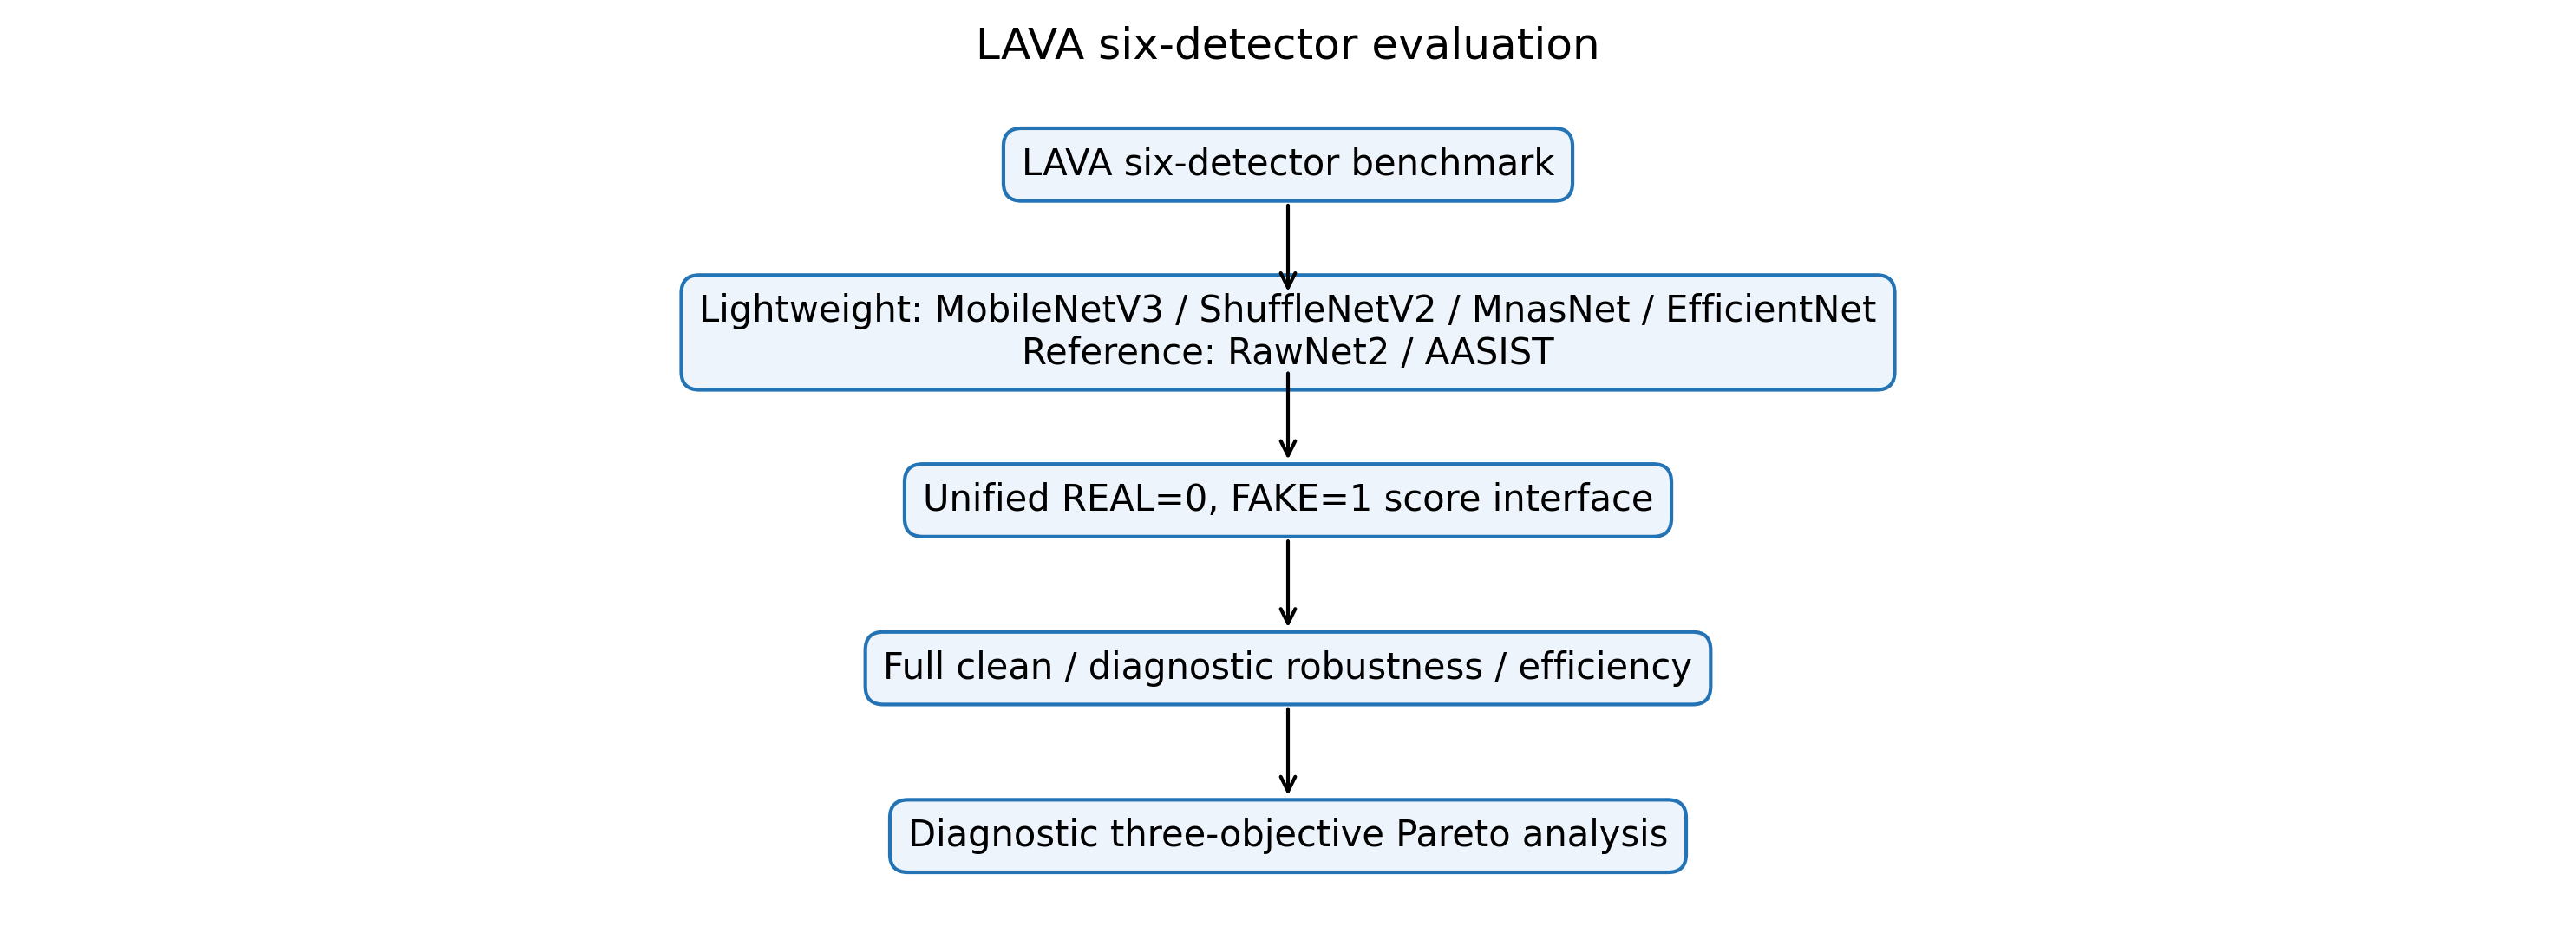
\includegraphics[width=.86\textwidth]{lava_6_model_overview.png}
\caption{Sáu bộ phát hiện nguyên bản được kết nối với ranh giới đánh giá thống nhất của LAVA.}
\label{fig:overview}
\end{figure}

\subsection{Tính toàn vẹn dữ liệu và phân hoạch chính tắc}
Bộ dữ liệu nhị phân nội bộ không có định danh người nói, nguồn, bộ sinh, bản ghi gốc hay tập dữ liệu; do đó LAVA không tuyên bố tính độc lập theo người nói, nguồn, bộ sinh hoặc tập dữ liệu. Hệ thống đã quét 18.722 tệp (10.550 REAL, 8.172 FAKE), phát hiện 435 nhóm trùng lặp và 476 tệp dư thừa, đồng thời cách ly toàn bộ 30 tệp thuộc 14 nhóm checksum khác nhãn. Trong một nhóm cùng nhãn, đường dẫn đứng đầu theo thứ tự từ điển được chọn làm đại diện chính tắc. 18.232 bản ghi được giữ lại gồm 10.493 REAL và 7.739 FAKE, được chia với seed 42 thành 12.762/2.733/2.737 mẫu huấn luyện/xác thực/kiểm thử. Tuyên bố được hỗ trợ chỉ là \emph{không giao nhau theo nhóm checksum}. Với $h(x)=\mathrm{SHA256}(x)$ và các tập nhóm phân hoạch $G_s$,
\begin{equation}
x_i\sim x_j\!\iff\!h(x_i)=h(x_j),\qquad G_{tr}\cap G_{va}=G_{tr}\cap G_{te}=G_{va}\cap G_{te}=\varnothing .
\label{eq:integrity}
\end{equation}
Hash manifest là \nolinkurl{8b55591d58d3658b8cafe0e77b6ebdedbaa67be2e339730a7276fe9b10958df9}. Hình~\ref{fig:integrity} và Bảng~\ref{tab:data} ghi lại một lần chính sách đã triển khai.

Trường hợp đồng nhất nhưng khác nhãn được xử lý thận trọng hơn trùng lặp thông thường: mọi thành viên của nhóm checksum xung đột đều bị loại, bởi chọn đại diện theo thứ tự từ điển sẽ tùy tiện giữ lại một nhãn không tương thích. Nhóm cùng nhãn giữ một đại diện để tránh gán trọng số nhiều lần cho các byte giống hệt nhau. Việc phân bổ phân hoạch vận hành trên nhóm checksum thay vì đường dẫn; trình kiểm tra manifest tính lại cả xung đột nhãn lẫn giao của từng cặp phân hoạch. Giao thức này ngăn rò rỉ ở mức byte nhưng không thể phát hiện bản mã hóa lại tương đồng về cảm nhận hoặc người nói dùng chung nếu không có metadata bổ sung.

\begin{figure}[!t]
\centering
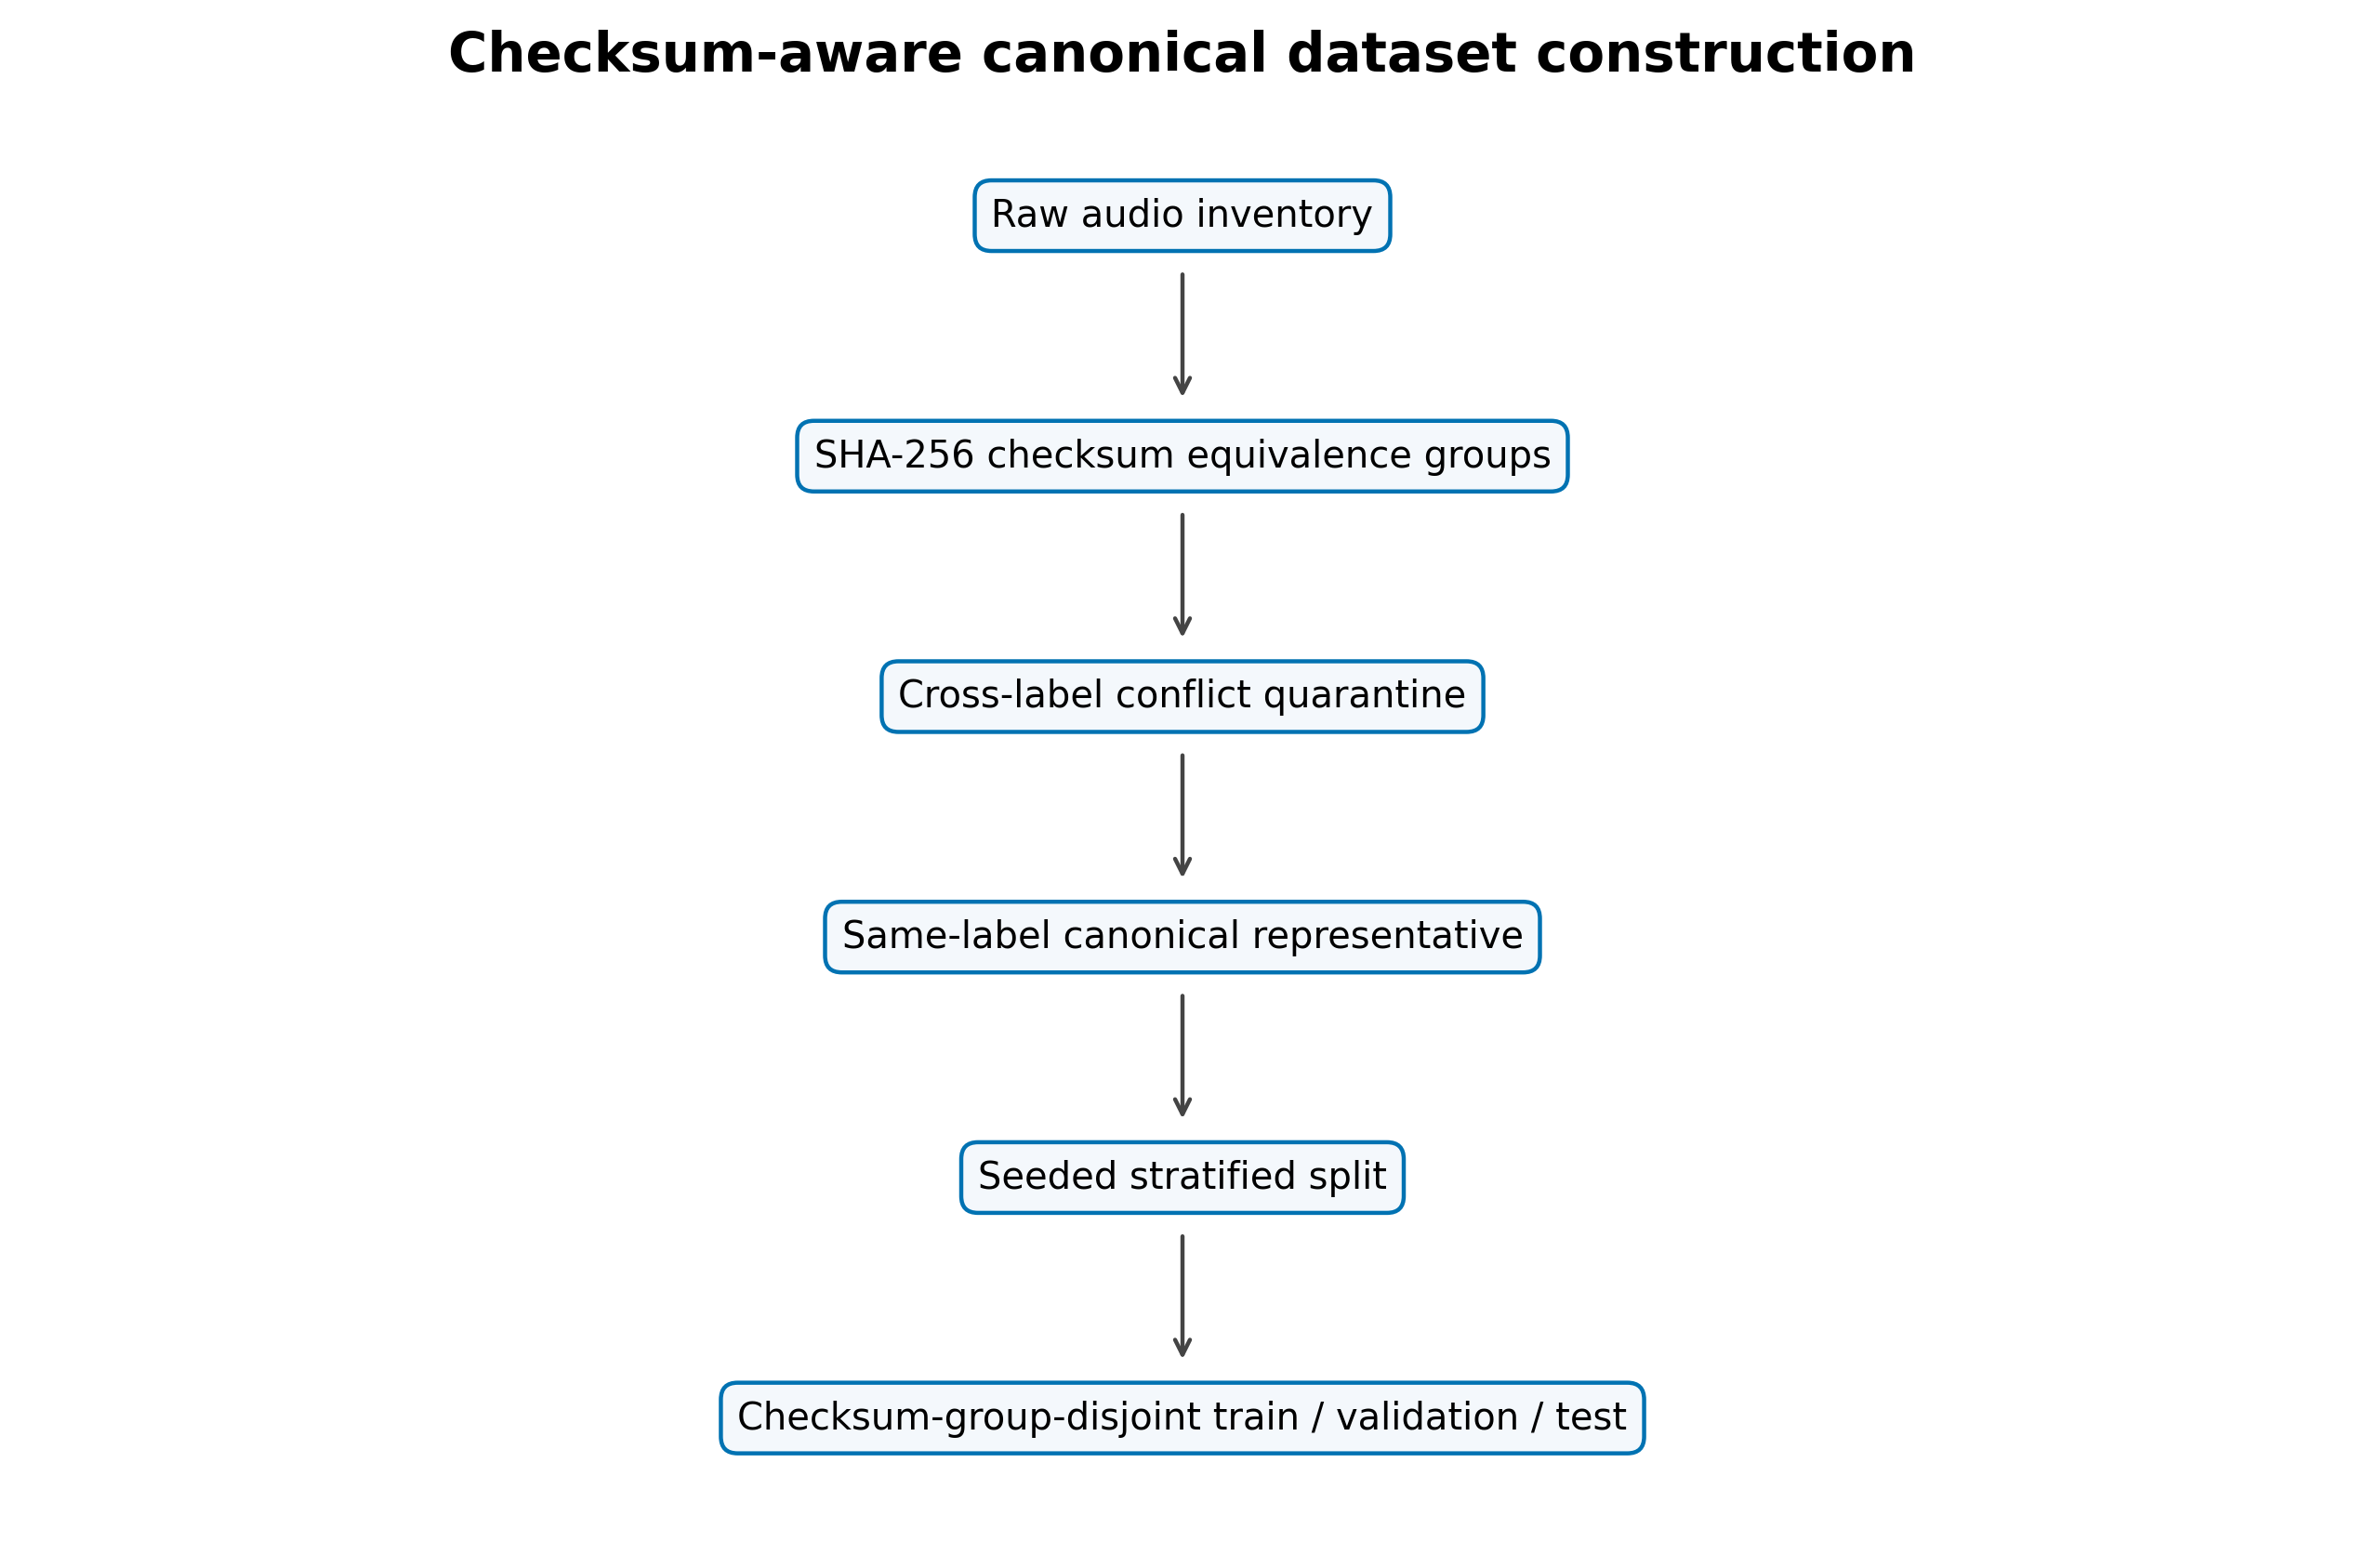
\includegraphics[width=.82\textwidth]{dataset_integrity_pipeline.png}
\caption{Cách ly xung đột SHA-256, chính tắc hóa và phân hoạch không giao nhau.}
\label{fig:integrity}
\end{figure}

\begin{table}[!t]
\centering\footnotesize
\caption{Kiểm kê manifest và phân hoạch chính tắc.}
\label{tab:data}
\begin{tabularx}{\textwidth}{Y r Y r}
\toprule
Hạng mục kiểm kê & Số lượng & Phân hoạch & Số lượng \\
\midrule
Đã quét / giữ lại & 18,722 / 18,232 & Huấn luyện & 12,762 \\
REAL / FAKE giữ lại & 10,493 / 7,739 & Xác thực & 2,733 \\
Nhóm trùng / tệp dư thừa & 435 / 476 & Kiểm thử & 2,737 \\
Nhóm / tệp khác nhãn & 14 / 30 & Tính độc lập & nhóm checksum \\
\bottomrule
\end{tabularx}
\end{table}

\subsection{Tiền xử lý âm thanh chuẩn hóa}
Đầu vào của các mô hình nhẹ được giải mã, lấy trung bình giữa các kênh, tái lấy mẫu đa pha về 22.050 Hz, rồi đệm hoặc cắt về 3,0 s. Sáu đoạn liên tiếp theo thời gian, mỗi đoạn 0,5 s, sử dụng STFT cửa sổ Hann ($N=2048$, bước nhảy 512), 128 bộ lọc Mel kiểu HTK trong dải 20--8.000 Hz, ánh xạ dB tương đối cắt tại 80 dB, co giãn về $[0,255]$, thay đổi kích thước song tuyến tính thành $224\times224$ và sao chép sang ba kênh RGB. Với đoạn $t$,
\begin{equation}
X_t(m,k)=\sum_{n=0}^{N-1}x_t[n+mH]w[n]e^{-j2\pi kn/N},\quad S_{t}^{mel}(m,r)=\sum_k|X_t(m,k)|^2H_r(k).
\label{eq:mel}
\end{equation}
Triển khai SciPy/Mel tường minh chỉ sử dụng librosa như phương án dự phòng khi giải mã \cite{mcfee2015librosa}. Ngược lại, các adapter tham chiếu tiếp nhận dạng sóng mono 16 kHz gồm 64.600 mẫu (4,0375 s), dùng phần tiền tố và đệm số không. Khác biệt đã được ghi nhận này được giữ nguyên thay vì mô tả sai thành tiền xử lý đồng nhất.

Chuẩn hóa tất định diễn ra trước khi chia sáu đoạn nên thứ tự thời gian không bao giờ bị xáo trộn. Giá trị dB của mỗi đoạn được quy chiếu theo cực đại của chính đoạn đó và được chặn dưới trước phép biến đổi logarit; tensor ảnh thu được có hình dạng $6\times224\times224\times3$ ở kiểu float32. Nhánh xác thực và kiểm thử không áp dụng tăng cường ngẫu nhiên. Cách đệm trong repository tham chiếu có thể khác cơ chế lấy tiền tố/đệm số không của LAVA đối với clip ngắn; vì vậy, tính tương đương giữa checkpoint bản địa và ONNX chỉ xác minh độ trung thực khi xuất mô hình trên cùng tensor adapter, không chứng minh tương đương với toàn bộ quy trình tiền xử lý của tác giả gốc.

\subsection{Kiến trúc các bộ phát hiện được đánh giá}
Đối với họ mô hình nhẹ, encoder đoạn dùng chung $f_\theta$ tạo sáu embedding, một LSTM 128 đơn vị tổng hợp chúng, sau đó lớp ReLU 64 đơn vị và dropout 0,4 cung cấp đầu vào cho sigmoid:
\begin{equation}
p_{fake}=\sigma\!\left(W_2\,\mathrm{Dropout}_{.4}\!\left(\mathrm{ReLU}(W_1\mathrm{LSTM}(f_\theta(X_{1:6}))+b_1)\right)+b_2\right).
\label{eq:head}
\end{equation}
MobileNetV3 sử dụng phần dư đảo và các khối squeeze--excitation; ShuffleNetV2 dùng tách/trộn kênh; MnasNet cung cấp các tầng phần dư đảo được tìm kiếm có xét nền tảng; EfficientNet-B0 sử dụng co giãn hợp thành và các khối MBConv. RawNet2 giữ nguyên front-end kiểu Sinc, các khối phần dư, attention, GRU và bộ phân loại; AASIST giữ nguyên attention đồ thị dị thể theo phổ--thời gian và khối đọc đầu ra. Hình~\ref{fig:archprov} kết hợp đường xử lý nhẹ dùng chung với nguồn gốc không đồng nhất, một điều kiện bắt buộc khi diễn giải so sánh.

Kích thước embedding của backbone không bị ép bằng nhau: MobileNetV3 xuất 576 chiều, ShuffleNetV2 1.024 chiều, còn MnasNet/EfficientNet 1.280 chiều. TimeDistributed dùng chung một backbone cho cả sáu đoạn nên số tham số không tăng gấp sáu, dù khối lượng phép tích chập trên mỗi bản ghi có tăng. RawNet2 học trực tiếp từ các mẫu dạng sóng thông qua ngân hàng bộ lọc kiểu Sinc và hệ phân cấp phần dư theo thời gian trước khi GRU phân loại. AASIST xây dựng đồ thị phổ và thời gian, thực hiện attention đồ thị cùng tương tác dị thể với các nút chủ, rồi pooling để phân loại. LAVA không biến đổi cấu trúc tham chiếu nào thành Mel-CNN-LSTM.

MobileNetV3Small kết hợp nút thắt phần dư đảo với squeeze--excitation và các hàm phi tuyến có xét phần cứng, đồng thời tạo embedding đoạn hẹp nhất. Các đơn vị stride một của ShuffleNetV2 bảo toàn một nhánh kênh trong khi biến đổi nhánh còn lại bằng chuỗi tích chập pointwise/depthwise/pointwise; phép nối và trộn kênh trao đổi đặc trưng, còn đơn vị stride hai biến đổi cả hai nhánh. MnasNet-A1 và EfficientNet-B0 đều sử dụng nút thắt đảo dành cho thiết bị di động nhưng bắt nguồn từ tiêu chí tìm kiếm/co giãn khác nhau. Các chi tiết triển khai này quan trọng vì bốn backbone dùng chung một đầu hồi quy không đồng nghĩa với cùng dung lượng hay cảnh quan tối ưu hóa.

Họ tham chiếu chủ ý tạo thành một tầng so sánh khác biệt. Front-end giới hạn băng học được, các khối phần dư theo thời gian, attention kênh và GRU của RawNet2 hoạt động trên 64.600 mẫu. AASIST hình thành đặc trưng hai chiều, đồ thị phổ và thời gian, tương tác đồ thị dị thể, các nút chủ và graph pooling trước bộ phân loại. Repository nguồn liên kết các checkpoint này với ASVspoof 2019 LA, nhưng không mô hình nào được huấn luyện từ đầu bằng phân hoạch huấn luyện chính tắc của LAVA. Do đó, xuyên suốt nghiên cứu, chúng được mô tả là artifact chống giả mạo tham chiếu được tiền huấn luyện bên ngoài.

\begin{figure}[!t]
\centering
\begin{minipage}{.49\textwidth}\centering
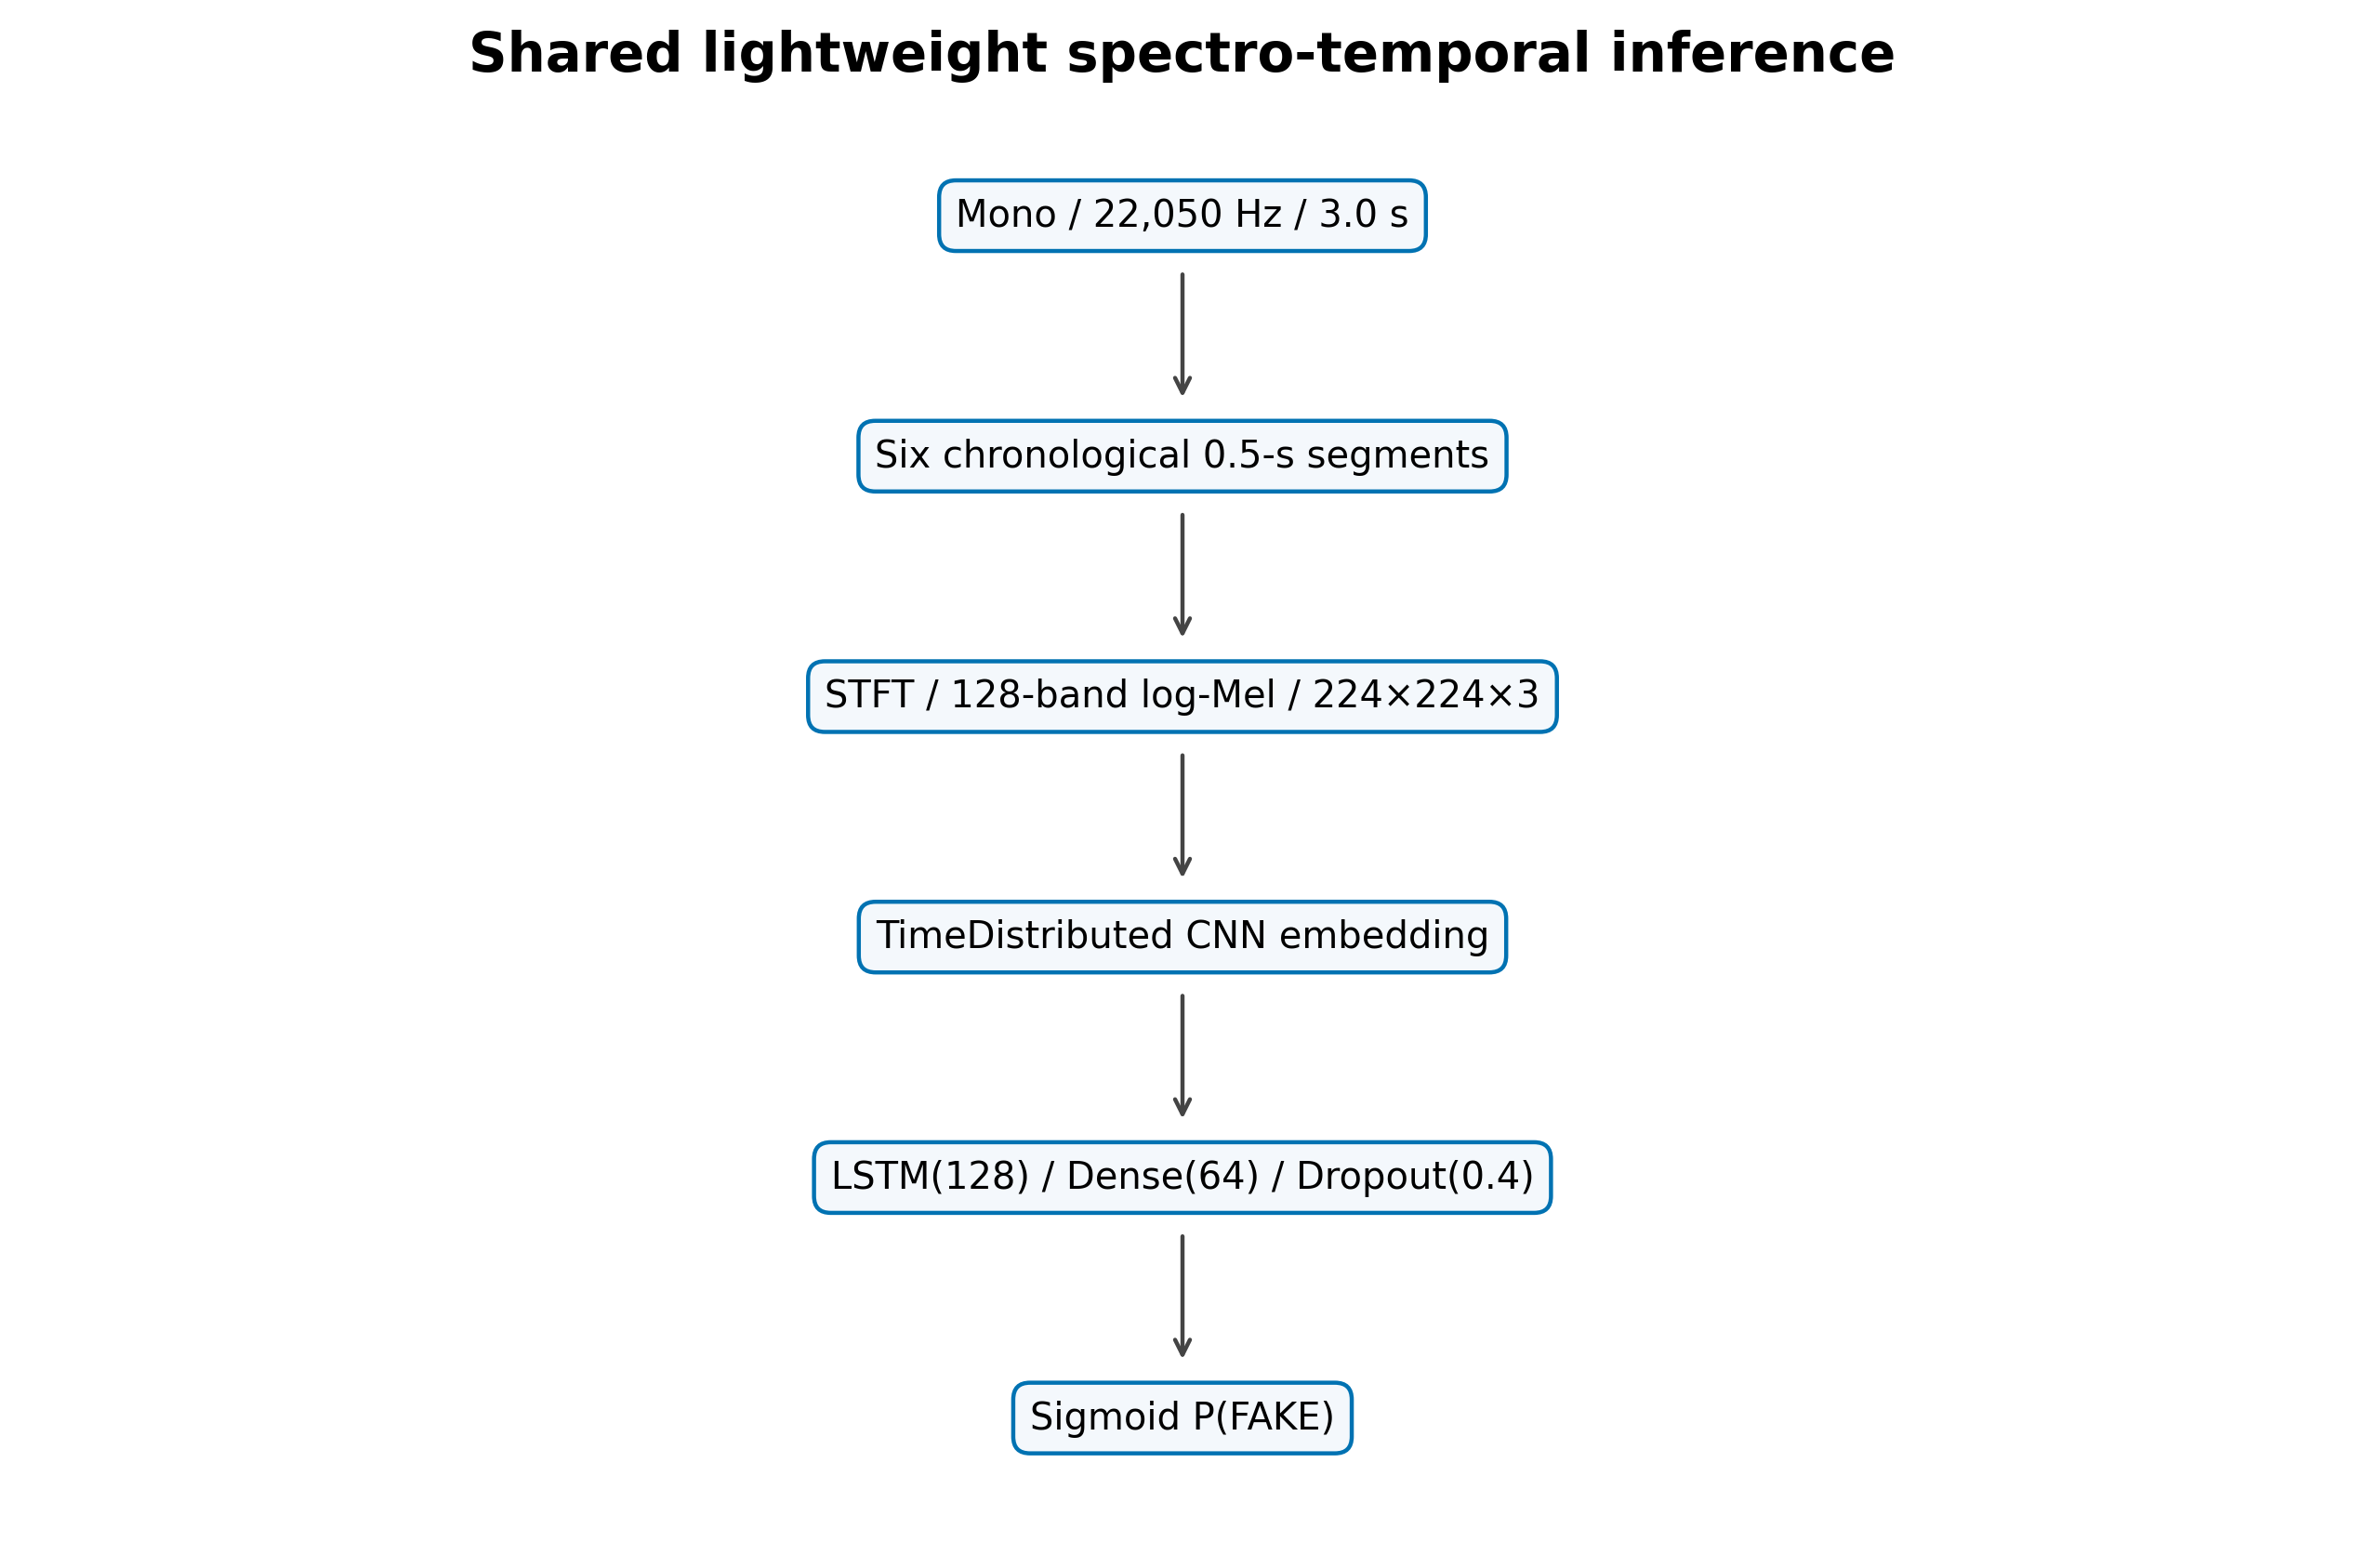
\includegraphics[width=\linewidth]{lightweight_temporal_pipeline.png}\\[-1mm]\small (a) Đường xử lý chuỗi Mel theo thời gian
\end{minipage}\hfill
\begin{minipage}{.49\textwidth}\centering
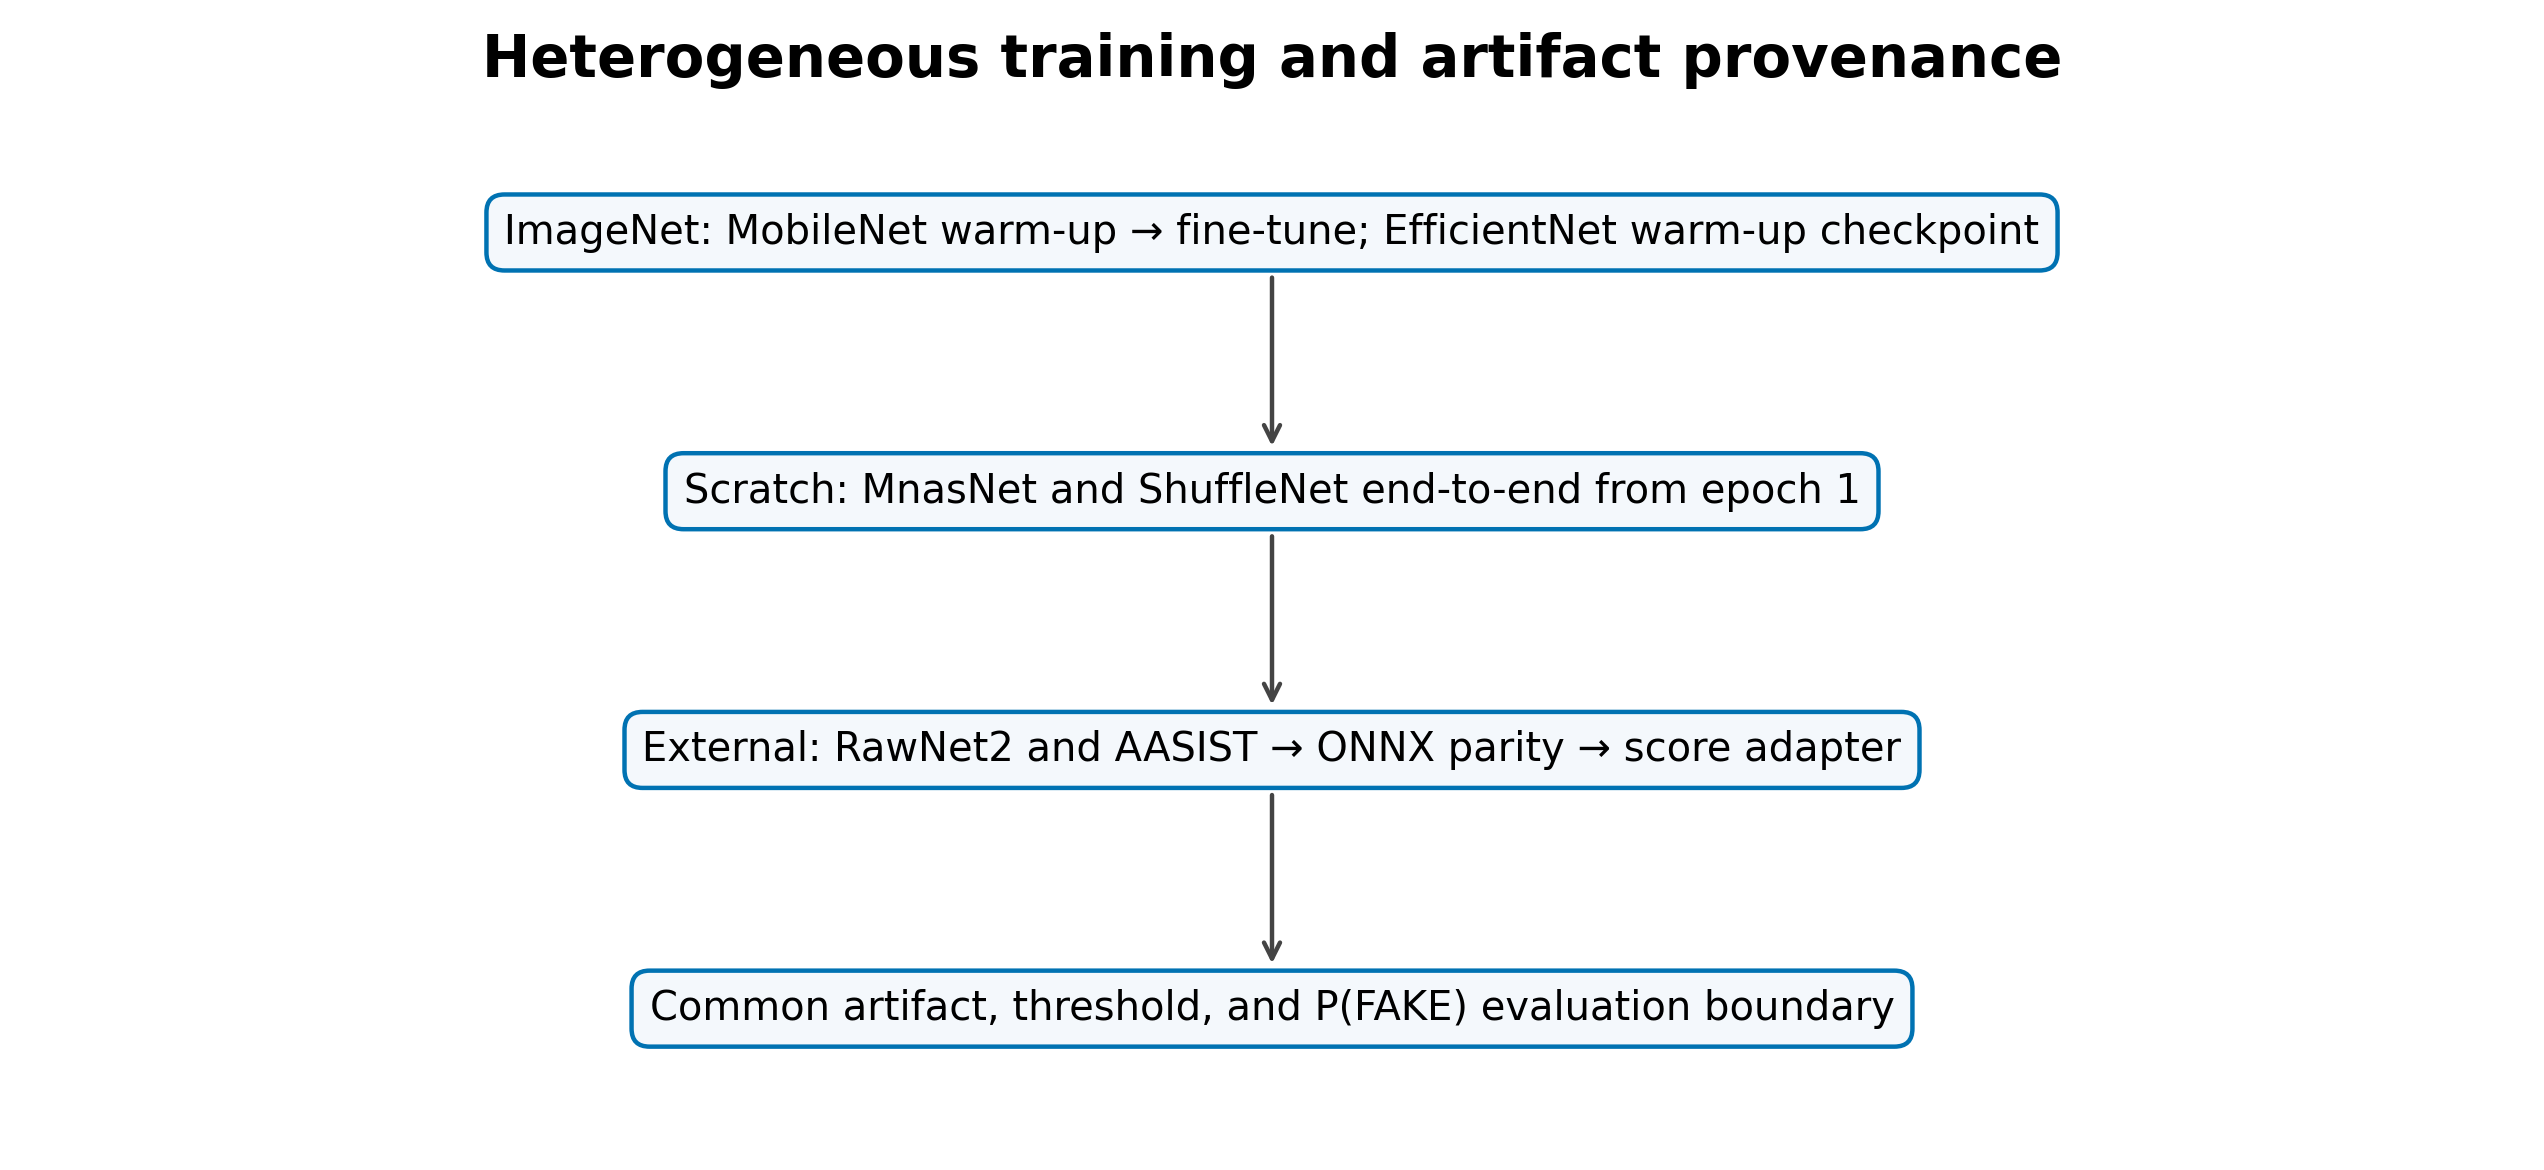
\includegraphics[width=\linewidth]{training_provenance_strategies.png}\\[-1mm]\small (b) Nguồn gốc artifact
\end{minipage}
\caption{Kiến trúc và nguồn gốc: hợp đồng đánh giá dùng chung nhưng quá trình huấn luyện thì không.}
\label{fig:archprov}
\end{figure}

\begin{table}[!t]
\centering
\scriptsize
\caption{Đặc tả bộ phát hiện, nguồn gốc và ngưỡng triển khai.}
\label{tab:models}

\begin{tabular*}{\textwidth}{
@{\extracolsep{\fill}}
l
l
l
r
p{0.39\textwidth}
r
}
\toprule
Bộ phát hiện & Đầu vào & Lõi thời gian & Tham số &
Khởi tạo/nguồn gốc artifact & $\tau$ \\
\midrule

MobileNetV3-LSTM
& Mel, 3.0 s
& LSTM(128)
& 1,308,401
& ImageNet; warm-up + fine-tune một phần
& .82 \\

ShuffleNetV2-LSTM
& Mel, 3.0 s
& LSTM(128)
& 1,868,441
& từ đầu; đầu cuối toàn phần, tốt nhất epoch 16/28
& .12 \\

MnasNet-A1-LSTM
& Mel, 3.0 s
& LSTM(128)
& 3,369,255
& từ đầu; đầu cuối toàn phần, tốt nhất epoch 27/39
& .90 \\

EfficientNet-B0-LSTM
& Mel, 3.0 s
& LSTM(128)
& 4,779,300
& ImageNet; warm-up tốt nhất epoch 47
& .90 \\

RawNet2
& dạng sóng, 4.04 s
& GRU
& 17,621,410
& tham chiếu ngoài; xuất ONNX
& .50 \\

AASIST
& dạng sóng, 4.04 s
& đọc đầu ra đồ thị
& 297,866
& tham chiếu ngoài; xuất ONNX
& .50 \\

\bottomrule
\end{tabular*}
\end{table}

\subsection{Huấn luyện, nguồn gốc artifact và ngữ nghĩa điểm số}
MobileNet và EfficientNet sử dụng khởi tạo ImageNet; artifact triển khai của EfficientNet được xác định rõ là checkpoint warm-up tốt nhất, không phải kết quả của một vòng đời fine-tune hoàn tất. MnasNet và ShuffleNet được huấn luyện từ đầu cùng với đầu hồi quy; lần lượt toàn bộ 49 và 56 lớp BatchNormalization có thể huấn luyện từ epoch 1. RawNet2 và AASIST không được LAVA huấn luyện: việc tải nghiêm ngặt bằng PyTorch rồi xuất ONNX cho sai khác điểm số bản địa/bản xuất tối đa là $4.11\times10^{-6}$ và $5.96\times10^{-8}$ trên sáu tensor thực. Kết quả này xác minh phép chuyển đổi, không chứng minh huấn luyện đồng nhất hay tương đương với pipeline trong công bố gốc.

MobileNet trải qua warm-up với backbone đóng băng, sau đó fine-tune một phần ở tốc độ học thấp hơn và vẫn đóng băng BatchNormalization. Checkpoint warm-up được chọn của EfficientNet ở epoch 47 (validation loss 0,1698). MnasNet dùng Adam từ $10^{-4}$, dừng ở epoch 39 và khôi phục epoch 27. ShuffleNet dùng Adam từ $3\times10^{-4}$, dừng ở epoch 28 và khôi phục epoch 16; backbone và toàn bộ lớp BatchNormalization vẫn có thể huấn luyện. Vì vậy, ranh giới đánh giá chung cung cấp phép kiểm thử tương ứng, không phải một so sánh có kiểm soát về khởi tạo hay tối ưu hóa.

LAVA cố định REAL=0 và FAKE=1; mọi adapter trả về $p=P(\mathrm{FAKE})$ và
\begin{equation}
\hat y=\mathbf{1}[p\ge\tau],\qquad \tau^*=\arg\max_{\tau}F1_{val}(\tau).
\label{eq:decision}
\end{equation}
Bốn ngưỡng của mô hình nhẹ trong Bảng~\ref{tab:models} chỉ sử dụng dữ liệu xác thực. Các mô hình tham chiếu bên ngoài giữ ngưỡng mặc định 0,5 chưa hiệu chỉnh. Nhãn kiểm thử không được dùng để chọn ngưỡng hoặc trọng số; các điểm số cũng không được tuyên bố là xác suất thực tế đã hiệu chỉnh.

Hiệu chỉnh ngưỡng tối đa hóa F1 của lớp FAKE trên lưới cấu hình bằng dữ liệu xác thực và được lưu cạnh artifact. Do đó, một điểm thấp hơn ngưỡng cao có thể được gán nhãn REAL ngay cả khi $p>0,5$; giao diện báo điểm thô và ranh giới quyết định thay vì trình bày $1-p$ như độ tin cậy đã hiệu chỉnh. ROC-AUC luôn được tính từ $P(\mathrm{FAKE})$ thô; EER cũng độc lập với ngưỡng tại điểm vận hành triển khai. Các quy ước này tránh âm thầm đảo thứ tự lớp bản địa: sigmoid TensorFlow vốn biểu diễn FAKE, còn adapter tham chiếu chọn chỉ số giả mạo do checkpoint xác định trước khi công bố điểm chung.

\subsection{Đánh giá sạch và độ bền vững}
Đánh giá sạch sử dụng toàn bộ 2.737 mẫu kiểm thử (1.575 REAL, 1.162 FAKE). Nghiên cứu báo cáo accuracy, F1 theo lớp và macro, ROC-AUC từ điểm thô và EER nội suy tuyến tính. Với FAKE là lớp dương,
\begin{equation}
P=\frac{TP}{TP+FP},\ R=\frac{TP}{TP+FN},\ F1=\frac{2PR}{P+R};\quad FAR=\frac{FP}{FP+TN},\ FRR=\frac{FN}{FN+TP},\ EER\simeq\frac{FAR+FRR}{2}.
\label{eq:metrics}
\end{equation}
Triển khai EER sắp xếp các ngưỡng điểm thô phân biệt, hình thành FAR và FRR, tìm lần đổi dấu đầu tiên của $FAR-FRR$, rồi nội suy tuyến tính tại giao điểm; nếu không có đổi dấu, hệ thống dùng khoảng cách tuyệt đối nhỏ nhất. Số đếm trong ma trận nhầm lẫn dùng ngưỡng triển khai đã lưu nên phụ thuộc điểm vận hành, trong khi ROC-AUC và EER đặc trưng cho thứ tự điểm số. Macro-F1 gán trọng số bằng nhau cho REAL và FAKE, bổ sung cho F1 lớp dương dùng khi chọn ngưỡng mô hình nhẹ.

Đánh giá độ bền vững sử dụng một tập con phân tầng 100 bản ghi kiểm thử được chọn trước (58 REAL, 42 FAKE; seed 42), và mỗi đường cơ sở dùng đúng các ID này. Bốn mức AWGN có seed (20, 10, 5, 0 dB) dùng seed suy ra từ định danh mẫu. Các vòng mã hóa--giải mã FFmpeg gồm MP3 128/64 kb/s, Opus 64 kb/s và AAC 96 kb/s. Phát lại mô phỏng áp dụng các tap tại 0/17/43/89 ms với hệ số 1/0,45/0,25/0,12, chuẩn hóa bằng 1,82 và bộ lọc thông dải nhân quả bậc bốn 100--3.800 Hz. Đây không phải phát lại vật lý. Với chín điều kiện,
\begin{equation}
\Delta F1_k=F1_{clean}-F1_k,\qquad \overline{\Delta F1}=\frac{1}{9}\sum_{k=1}^{9}\Delta F1_k.
\label{eq:degradation}
\end{equation}
Suy giảm âm biểu thị cải thiện trên tập con nhỏ này và không tự động đồng nghĩa với độ bền vững. Phép gây nhiễu trên toàn bộ tập kiểm thử, phát lại vật lý và đánh giá dữ liệu chưa thấy lần lượt có trạng thái \texttt{NOT\_RUN}, \texttt{NOT\_AVAILABLE} và \texttt{NOT\_AVAILABLE}.

Công suất nhiễu được suy ra từ công suất đo của từng tín hiệu sạch; 16 ký tự thập lục phân đầu tiên trong định danh SHA-256 quyết định seed ngẫu nhiên. Dạng sóng gây nhiễu được tạo một lần và dùng chung cho mọi adapter. Âm thanh codec được chuyển sang PCM16, mã hóa, giải mã rồi đưa lại qua đường mô hình thông thường; phiên bản thư viện codec không được niêm phong nên được ghi là \texttt{NOT\_MEASURED}. Các biện pháp kiểm soát này tách khác biệt giữa bộ phát hiện khỏi các nhiễu được lấy mẫu hoặc mã hóa lại độc lập.

\subsection{Phân tích hiệu suất, thống kê và Pareto}
Mỗi artifact chạy ở float32, batch một, một luồng backend, không có bộ tăng tốc và trong tiến trình cô lập tuần tự trên cùng CPU máy tính để bàn Windows AMD64. Mười lượt warm-up diễn ra trước 50 lần lặp có đo thời gian. Phép đo tách thời gian tiền xử lý, chỉ mô hình và đầu cuối, đồng thời bao gồm P95, thời gian tải, thông lượng và RSS của toàn tiến trình. Tên thương mại của CPU và dung lượng RAM cài đặt không được ghi nhận. Với $N$ clip,
\begin{equation}
Q=\frac{N}{T_{total}},\qquad RTF=\frac{T_{processing}}{T_{audio}}.
\label{eq:efficiency}
\end{equation}
RTF nhỏ hơn một chứng minh xử lý ngoại tuyến nhanh hơn thời lượng âm thanh, không chứng minh xử lý luồng nhân quả hay triển khai biên.

Runner báo thời gian tiền xử lý và chỉ mô hình bên cạnh trung bình đầu cuối, P95, thông lượng, thời gian tải và RSS được lấy mẫu mỗi 20 ms. Thời gian khởi động trình thông dịch và trace đồ thị bị loại khỏi phép đo sau warm-up. Số tham số Keras bao gồm trạng thái BatchNormalization không thể huấn luyện, trong khi số đếm PyTorch bản địa của mô hình tham chiếu loại trừ buffer; vì vậy kích thước tuần tự hóa và độ trễ thực thi vẫn là các đại lượng được báo cáo riêng.

Các lần lặp chỉ mô hình và đầu cuối được warm-up độc lập. Phép đo thời gian đồng bộ thực thi bằng cách hiện thực hóa mảng trả về trước khi dừng đồng hồ, tránh nhầm việc điều phối bất đồng bộ với hoàn tất tính toán. Thông lượng là nghịch đảo của tổng thời lượng đầu cuối thay vì nghịch đảo của một giá trị trung bình đã làm tròn. Mẫu số RTF tuân theo thời lượng khai báo của từng bộ phát hiện (3,0 s cho mô hình nhẹ và 4,0375 s cho mô hình tham chiếu). Vì vậy, RTF hỗ trợ so sánh triển khai trong cùng giao thức nhưng không xóa bỏ khác biệt về thời lượng đầu vào.

Sáu tệp điểm số trên toàn bộ tập kiểm thử được nối theo ID mẫu. Một nghìn mẫu lặp bootstrap phân tầng theo lớp (seed 42) tạo khoảng phân vị 95\% cho F1, AUC và EER \cite{efron1979bootstrap}. Kiểm định McNemar chính xác so sánh tính đúng/sai theo cặp \cite{mcnemar1947}; hiệu chỉnh Holm bao quát toàn bộ 15 cặp \cite{holm1979}. Mức đồng thuận là tỷ lệ quyết định giống nhau. Đây là độ bất định do mẫu kiểm thử, không phải độ bất định đa seed. Các mục tiêu Pareto chẩn đoán tối thiểu hóa EER trên tập con, $\Delta F1$ trung bình và RTF đầu cuối. Mô hình $A$ trội hơn $B$ khi và chỉ khi
\begin{equation}
f_i(A)\le f_i(B)\ \forall i\quad\text{và}\quad\exists j:f_j(A)<f_j(B).
\label{eq:pareto}
\end{equation}
Không sử dụng điểm tổng hợp có trọng số. Vì độ bền vững chỉ bao quát 100 bản ghi, biên này mang tính thăm dò; biên chính thức trên toàn bộ tập kiểm thử vẫn có trạng thái \texttt{NOT\_RUN}. Điểm theo từng mẫu, hash, thống kê đầy đủ và script sinh kết quả được giữ trong phần bổ trợ của repository.

Lấy mẫu lại bootstrap bảo toàn số lượng lớp quan sát bằng cách lấy độc lập chỉ số REAL và FAKE rồi kết hợp lại, nên một mẫu lặp không thể vô tình mất một lớp. Khoảng sai khác F1 theo cặp dùng lại cùng các ID được lấy mẫu cho cả hai mô hình để bảo toàn tính phụ thuộc. McNemar chỉ đếm các kết quả đúng/sai bất đồng và kiểm tra tính đối xứng theo hướng; hiệu chỉnh tuần tự Holm kiểm soát sai số họ kiểm định mà không giả định các bộ phát hiện độc lập. Phân tích đồng thuận và phần lỗi giao nhau là bổ sung mô tả, không phải kiểm định ý nghĩa thống kê.

Khả năng tái lập được tổ chức quanh bằng chứng bất biến thay vì các con số chép vào bản thảo. Đầu ra sạch chính tắc chứa 2.737 hàng điểm cho mỗi bộ phát hiện tại \texttt{outputs/lava\_6/clean}; đầu ra độ bền vững giữ 100 ID mẫu đã chọn và manifest điều kiện; bản tóm tắt hiệu suất niêm phong số lượt warm-up/chạy và chính sách luồng. Bảng tổng hợp được sinh từ các tệp CSV/JSON này mà không import bộ tải mô hình, nên quá trình sinh bài báo không thể kích hoạt thực thi mô hình. Registry bộ phát hiện và giao diện production dùng metadata đã đóng gói khi đầu ra benchmark bị bỏ qua không tồn tại lúc triển khai. Kiểm tra nghiệm thu yêu cầu sáu hàng sạch và hiệu suất, sáu mục cho từng điều kiện gây nhiễu đã hoàn tất, ma trận đồng thuận $6\times6$ và sáu đầu vào Pareto. Đầu ra lịch sử năm mô hình không thay đổi, cho phép kiểm toán việc bổ sung ShuffleNet theo cách tăng dần.

Phạm vi sạch và chẩn đoán được chủ ý phân tách trong tên tệp, bản tóm tắt và cách diễn đạt. EER toàn bộ tập kiểm thử xuất hiện trong kết quả sạch và báo cáo bootstrap; EER tập con chỉ được dùng trong vector Pareto chẩn đoán vì tọa độ độ bền vững tương ứng dùng cùng 100 ID. Trộn EER toàn bộ tập với suy giảm trên tập con sẽ tạo một biên hợp lệ về số học nhưng không nhất quán về phạm vi. Tương tự, đường cơ sở sạch 100 mẫu không bao giờ thay thế bảng sạch 2.737 mẫu. Kỷ luật phạm vi này là một phần của hợp đồng benchmark, không chỉ là quy ước báo cáo.

\section{Kết quả và thảo luận}
\subsection{Hiệu năng phát hiện trên dữ liệu sạch (RQ1)}
Cả sáu artifact đều vượt qua kiểm tra tải, điểm số hữu hạn trong miền hợp lệ, hash và adapter. Bảng~\ref{tab:clean} báo cáo toàn bộ tập kiểm thử chính tắc. ShuffleNet dẫn đầu mọi chỉ số tổng hợp (F1 0,9824, macro-F1 0,9847, AUC 0,9929, EER 0,0146) với 24 dương tính giả và 17 âm tính giả. MobileNet đứng thứ hai về F1 và AUC, tiếp theo là MnasNet và checkpoint warm-up EfficientNet hiện có. RawNet2 và AASIST đạt mức gần ngẫu nhiên trong hợp đồng dataset/adapter này. Đây không phải xếp hạng chỉ theo kiến trúc vì nguồn gốc, thời lượng, biểu diễn, hiệu chỉnh ngưỡng và huấn luyện khác nhau.

Số đếm theo lớp làm rõ hơn bức tranh tổng hợp. MobileNet tạo 30 dương tính giả và 34 âm tính giả. MnasNet đánh đổi nhiều dương tính giả hơn (47) để có ít âm tính giả hơn (36); phân bố 31/69 của EfficientNet cho thấy lỗi chính là bỏ sót giọng FAKE tại ngưỡng được chọn bằng tập xác thực. RawNet2 tạo 1.015 dương tính giả và 371 âm tính giả; AASIST tạo 715 và 513. Các kết quả tham chiếu này phù hợp với khả năng lệch điểm số/miền và ngưỡng mặc định chưa hiệu chỉnh, nhưng bằng chứng hiện tại không thể quy nguyên nhân cho riêng một yếu tố.

Các giá trị F1 REAL/FAKE tương ứng là 0,9797/0,9724 cho MobileNet, 0,9870/0,9824 cho ShuffleNet, 0,9736/0,9645 cho MnasNet và 0,9686/0,9563 cho EfficientNet. Giá trị tham chiếu là 0,4469/0,5330 cho RawNet2 và 0,5834/0,5139 cho AASIST. Báo cáo cả hai lớp giúp F1 lớp dương không che khuất xu hướng bất đối xứng của RawNet2 khi gán nhãn FAKE cho bản ghi REAL. Số đếm nhầm lẫn và giá trị theo lớp vẫn có thể tái lập từ CSV điểm đầy đủ thay vì từ ảnh đã chuẩn hóa.

\begin{table}[!t]
\centering
\scriptsize
\caption{Hiệu năng sạch trên toàn bộ 2.737 bản ghi kiểm thử chính tắc.}
\label{tab:clean}

\begin{tabular*}{\textwidth}{
@{\extracolsep{\fill}}
l
r
r
r
r
r
r
r
}
\toprule
Mô hình & Acc. & Prec. & Rec. & F1 & Macro-F1 & AUC & EER \\
\midrule
MobileNetV3    & .9766 & .9741 & .9707 & .9724 & .9761 & .9911 & .0250 \\
ShuffleNetV2   & .9850 & .9795 & .9854 & .9824 & .9847 & .9929 & .0146 \\
MnasNet-A1     & .9697 & .9599 & .9690 & .9645 & .9690 & .9886 & .0310 \\
EfficientNet-B0& .9635 & .9724 & .9406 & .9563 & .9624 & .9877 & .0400 \\
RawNet2 ext.   & .4936 & .4380 & .6807 & .5330 & .4900 & .5178 & .4813 \\
AASIST ext.    & .5513 & .4758 & .5585 & .5139 & .5487 & .5597 & .4463 \\
\bottomrule
\end{tabular*}

\end{table}
Các đồ thị ROC và DET từ điểm thô trong Hình~\ref{fig:clean} tách khả năng phân biệt độc lập với ngưỡng khỏi quyết định triển khai. Bốn đường cong mô hình nhẹ thể hiện tốt; các đường tham chiếu gần đường chéo. Khoảng bootstrap giao nhau giữa một số hệ thống nhẹ, vì vậy các giá trị AUC gần nhau không được trình bày như thứ hạng phổ quát.

Kiểm tra artifact cũng giới hạn cách diễn giải khoảng cách này. Bản chuyển đổi TensorFlow 2.15 của ShuffleNet tái tạo điểm nguồn với sai khác trong $1.75\times10^{-10}$ và khớp hash manifest huấn luyện chính tắc. Các bản xuất ONNX tham chiếu khớp checkpoint bản địa trong dung sai báo cáo tại Mục III-E, khiến lỗi tuần tự hóa nghiêm trọng hoặc đảo chỉ số lớp khó xảy ra. Tuy nhiên, ngưỡng mô hình nhẹ được hiệu chỉnh trên tập xác thực và ngưỡng tham chiếu chưa hiệu chỉnh ảnh hưởng đến chỉ số nhầm lẫn; dịch chuyển miền và tiền xử lý ảnh hưởng cả phép đo dùng ngưỡng lẫn điểm thô. Do đó, kết quả hỗ trợ nhận định về artifact đã triển khai trong LAVA, không phải hiệu năng tối đa RawNet2 hoặc AASIST có thể đạt sau tái huấn luyện hay hiệu chỉnh.

\begin{figure}[!t]
\centering
\begin{minipage}{.49\textwidth}\centering
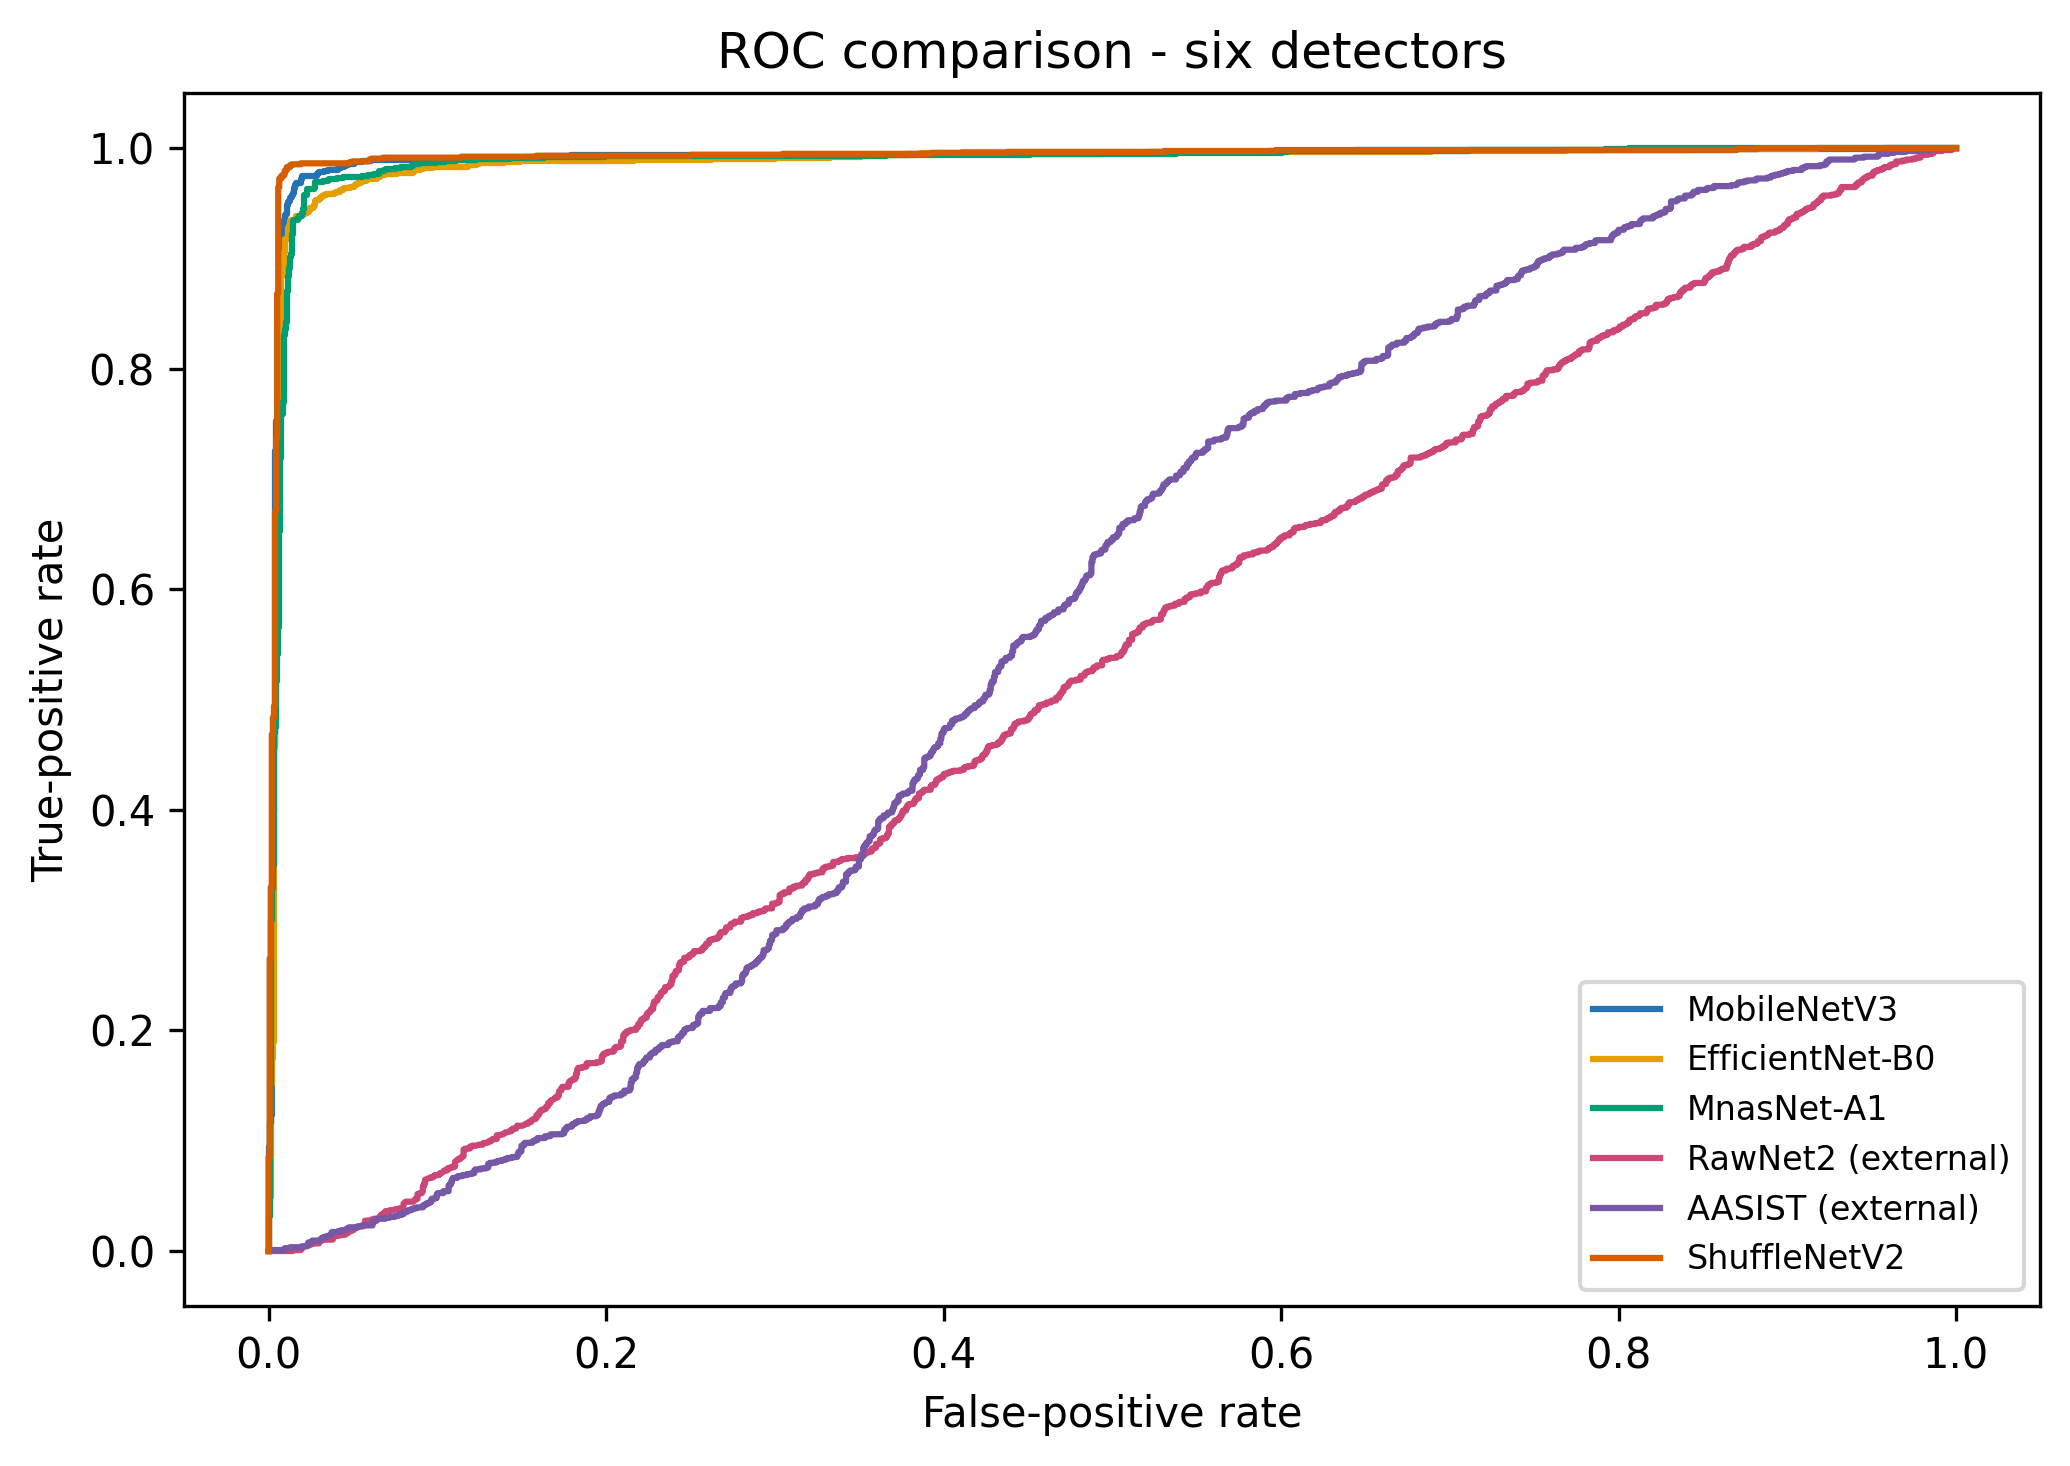
\includegraphics[width=\linewidth]{roc_comparison_6_models.png}\\[-1mm]\small (a) ROC
\end{minipage}\hfill
\begin{minipage}{.49\textwidth}\centering
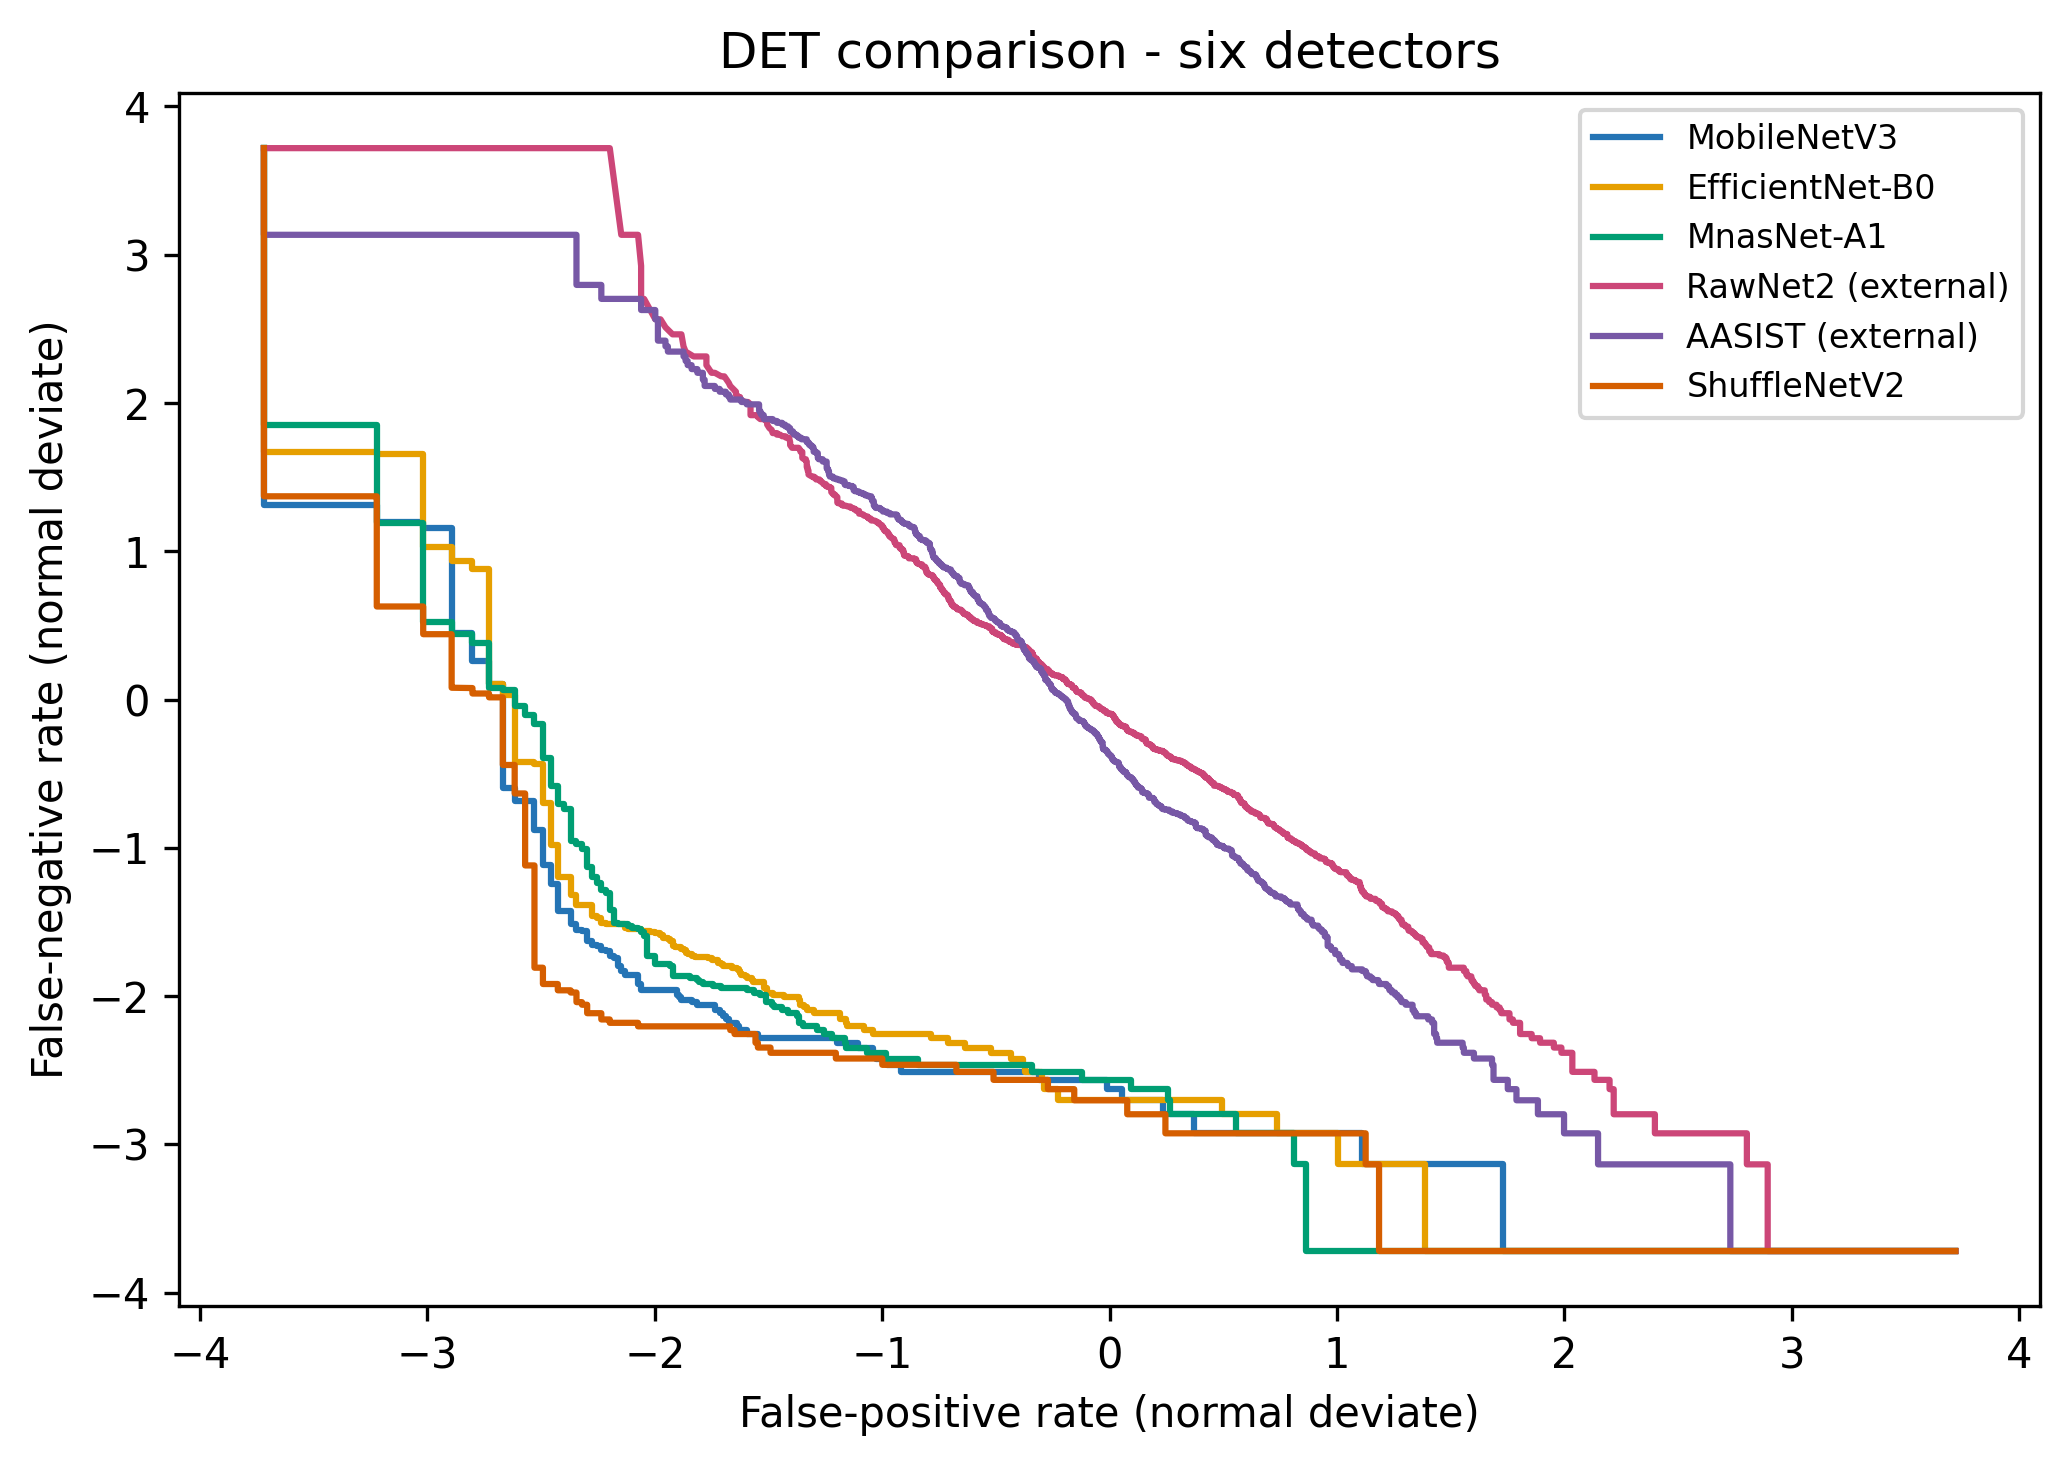
\includegraphics[width=\linewidth]{det_comparison_6_models.png}\\[-1mm]\small (b) DET/EER
\end{minipage}
\caption{Khả năng phân biệt sạch độc lập với ngưỡng trên toàn bộ phân hoạch kiểm thử.}
\label{fig:clean}
\end{figure}

\subsection{Độ bền vững dưới các biến dạng thực tiễn (RQ2)}
Bảng~\ref{tab:robustness} và Hình~\ref{fig:robustness} tóm tắt phép chẩn đoán ghép cặp. AWGN là điểm yếu lớn nhất đối với mọi hệ thống nhẹ có hiệu năng cao: suy giảm trung bình do nhiễu nằm trong khoảng 0,3555 của ShuffleNet đến 0,8053 của EfficientNet và tăng nhanh tại 5 và 0 dB. Thay đổi do codec nhỏ trong các cấu hình được thử nghiệm (0,0000--0,0233 trên các mô hình nhẹ). Dưới phát lại mô phỏng, ShuffleNet giữ F1 0,9500 ($\Delta$F1 0,0256), so với mức suy giảm 0,0620/0,0641/0,1489 của MobileNet/EfficientNet/MnasNet. Delta âm của mô hình tham chiếu bắt nguồn từ đường cơ sở thấp và sự phân bố lại điểm số; chúng không xác lập độ bền vững vượt trội.

\begin{table}[!t]
\centering
\footnotesize
\caption{Suy giảm F1 chẩn đoán trên tập con cố định 100 bản ghi; thấp hơn là tốt hơn.}
\label{tab:robustness}

\begin{tabular*}{\textwidth}{
@{\extracolsep{\fill}}
l
r
r
r
r
r
}
\toprule
Mô hình & F1 sạch & Nhiễu $\Delta$ & Codec $\Delta$ &
Phát lại $\Delta$ & Trung bình (9) \\
\midrule
MobileNetV3     & .9756 & .6722 & .0095 & .0620 & .3099 \\
ShuffleNetV2    & .9756 & .3555 & .0032 & .0256 & .1623 \\
MnasNet-A1      & .9756 & .6119 & .0233 & .1489 & .2989 \\
EfficientNet-B0 & .9630 & .8053 & .0000 & .0641 & .3650 \\
RawNet2 ext.    & .5660 & .5077 & $-.0007$ & $-.0109$ & .2241 \\
AASIST ext.     & .5060 & $-.0660$ & $-.0074$ & $-.0682$ & $-.0402$ \\
\bottomrule
\end{tabular*}

\end{table}

\begin{figure}[!t]
\centering
\begin{minipage}{.57\textwidth}\centering
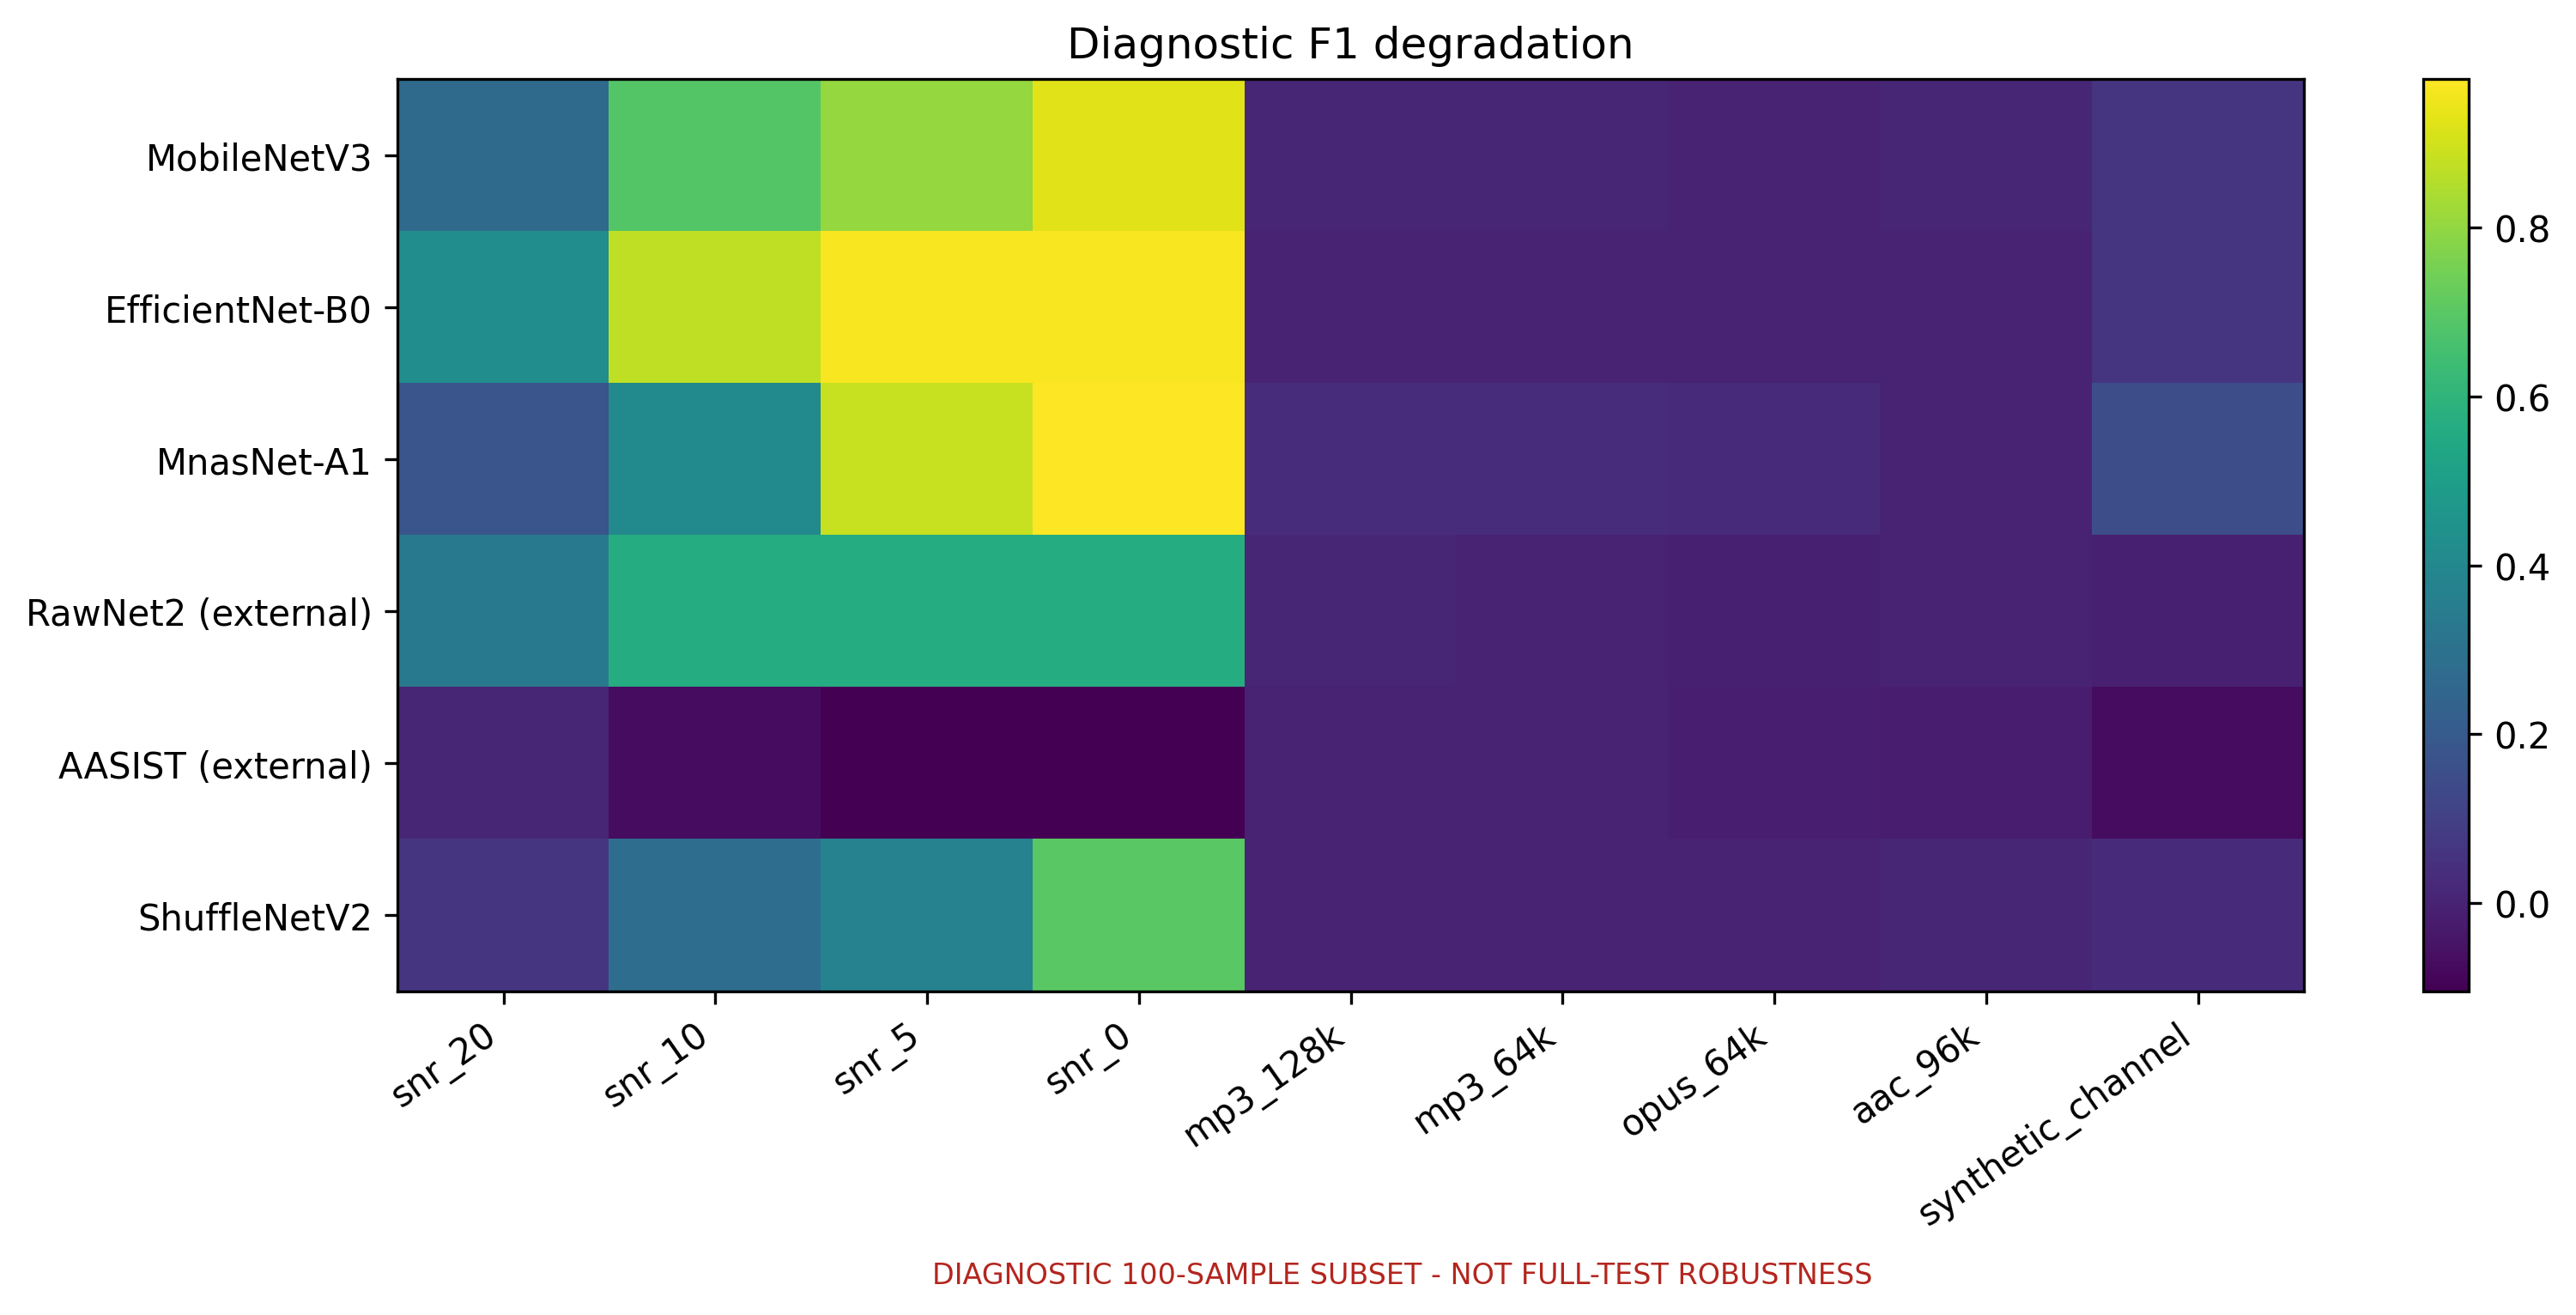
\includegraphics[width=\linewidth]{robustness_heatmap_6_models.png}\\[-1mm]\small (a) Suy giảm trên chín điều kiện
\end{minipage}\hfill
\begin{minipage}{.41\textwidth}\centering
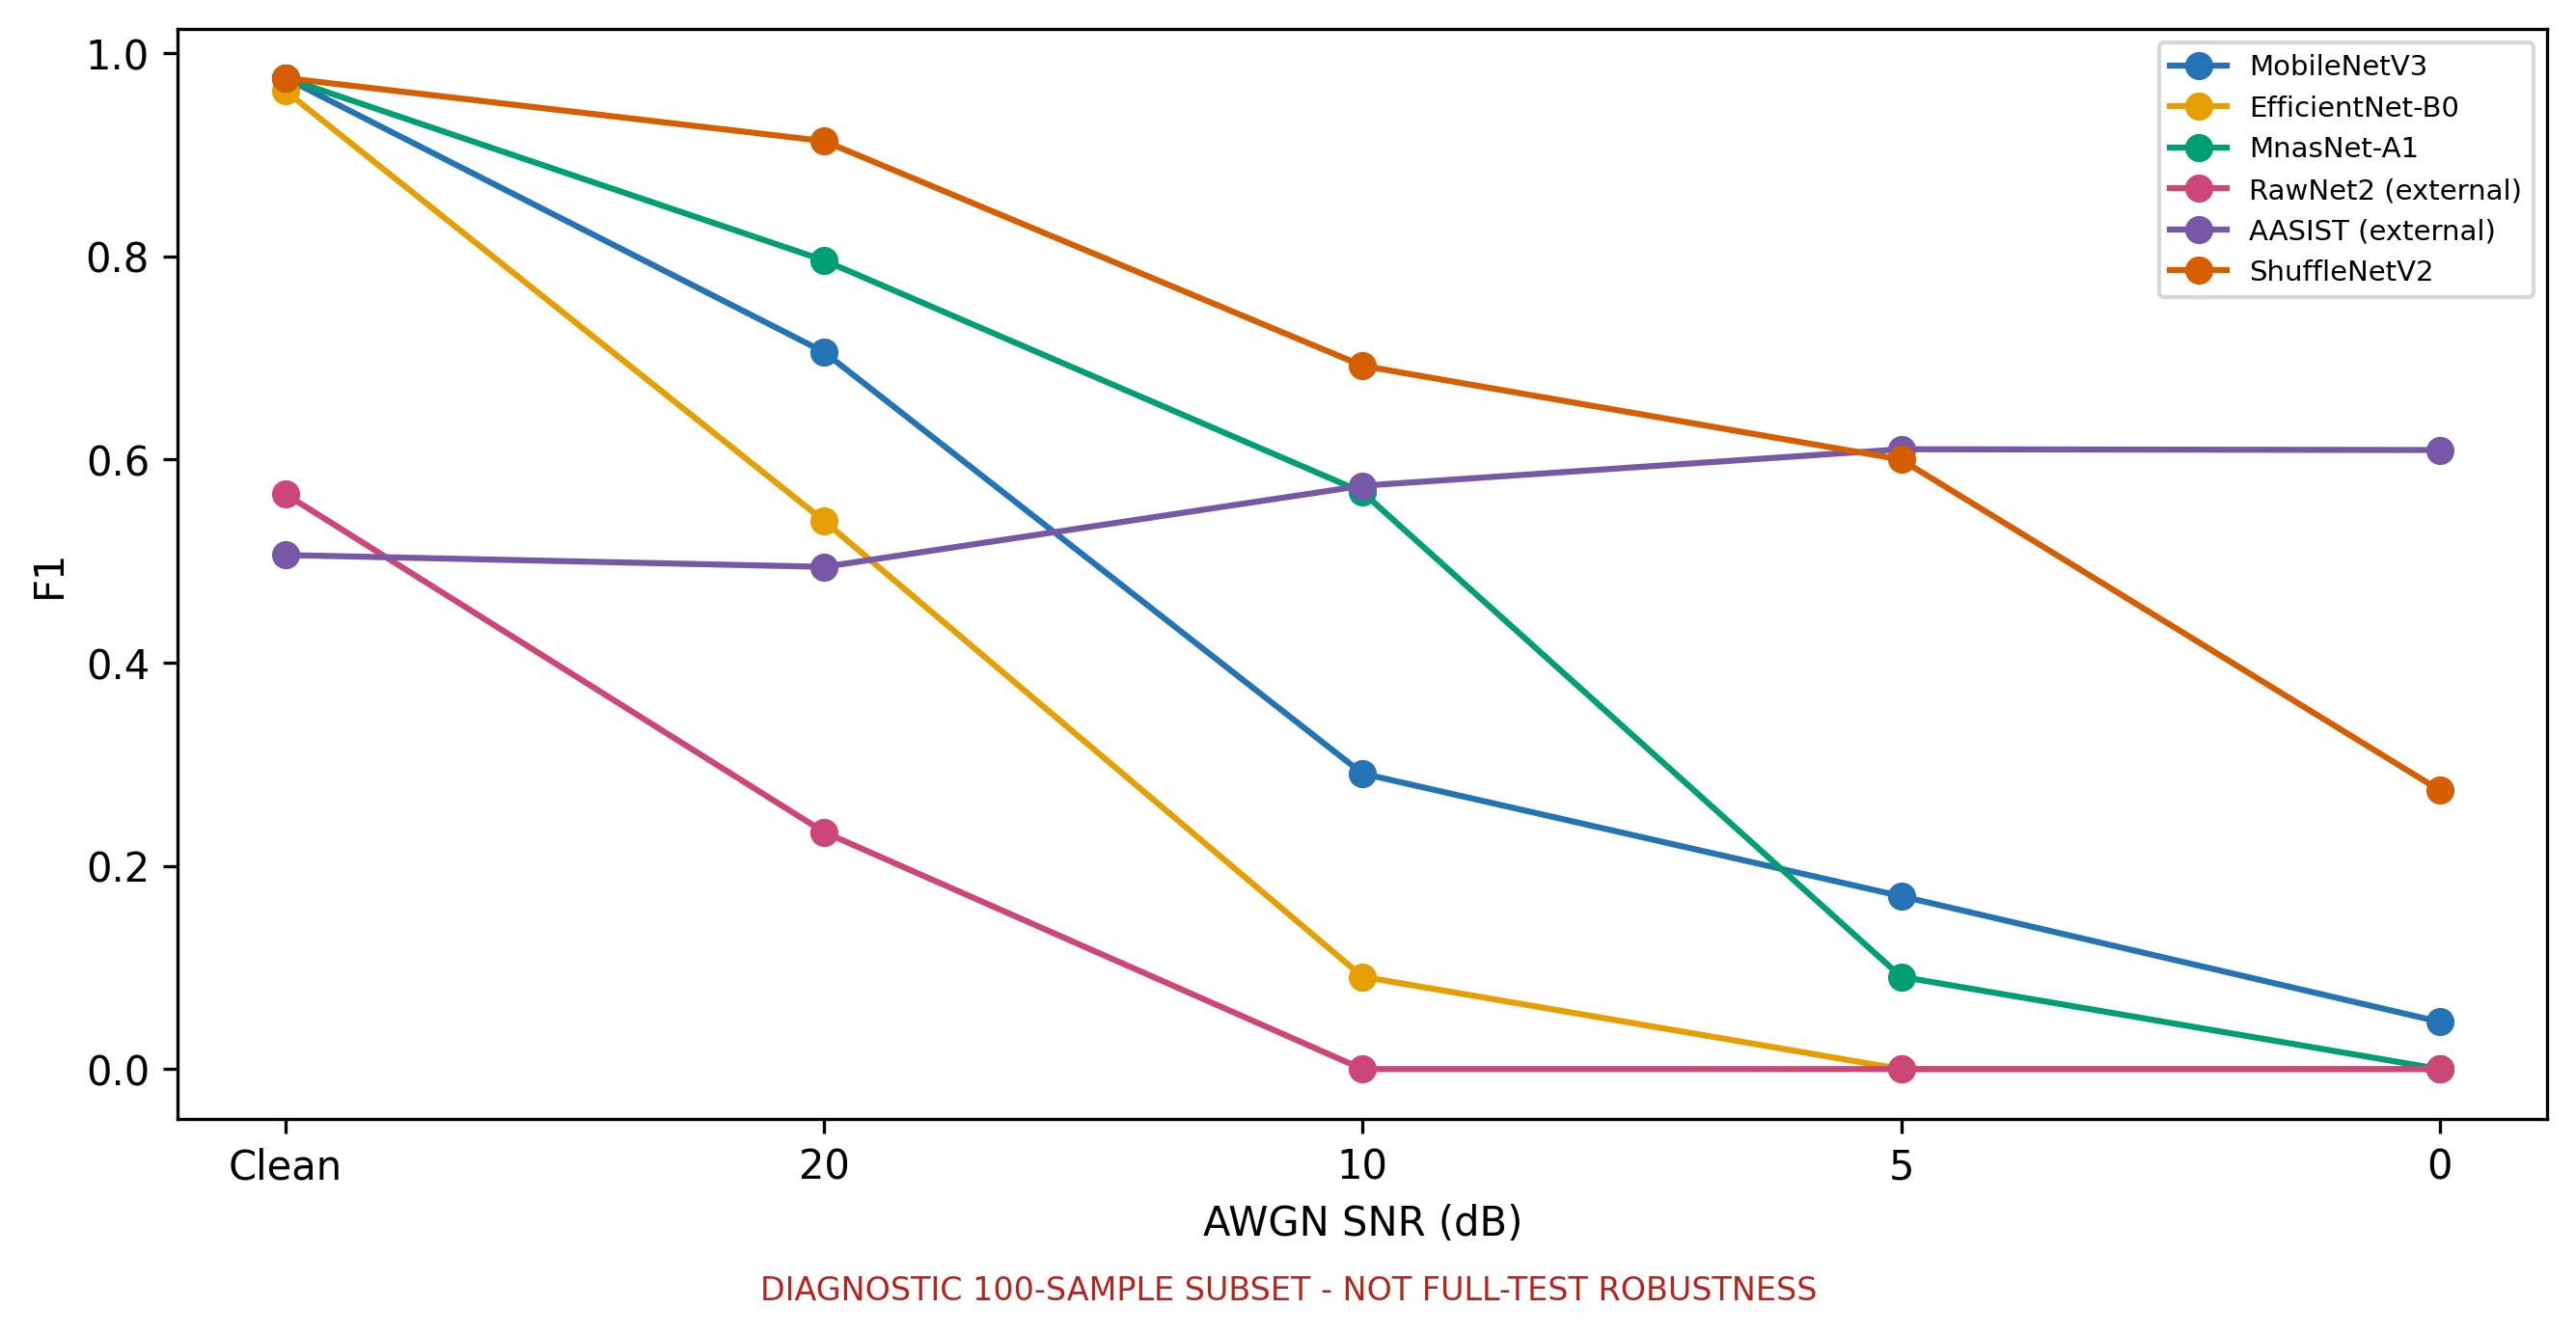
\includegraphics[width=\linewidth]{noise_f1_vs_snr_6_models.png}\\[-1mm]\small (b) Quỹ đạo F1 dưới AWGN
\end{minipage}
\caption{Độ bền vững chẩn đoán; mọi mô hình sử dụng lại các bản ghi gây nhiễu giống hệt nhau.}
\label{fig:robustness}
\end{figure}
Các kết quả này chỉ trả lời RQ2 trong phạm vi tập con và phép biến đổi đã thực thi. Tính ổn định trước codec không thể khái quát vượt ngoài bốn vòng mã hóa--giải mã, phát lại không phải vật lý và không tồn tại corpus chưa thấy.

Kiểm tra theo từng điều kiện ngăn giá trị trung bình theo nhóm che khuất các chuyển tiếp. F1 của mô hình nhẹ tương đối ổn định ở mức nhiễu nhẹ nhất nhưng giảm mạnh về phía 5 và 0 dB; thứ hạng cũng thay đổi theo SNR. Delta codec nhỏ không hàm ý bất biến với chuyển mã nói chung, bởi bitrate, triển khai encoder, tái lấy mẫu, mất gói và nén nối tiếp không được biến thiên. Tương tự, một đáp ứng xung tổng hợp duy nhất kiểm tra giới hạn băng và năng lượng trễ nhưng không bao quát đa dạng phòng, phi tuyến phát lại, đáp ứng microphone hay khoảng cách.

Trên cả chín điều kiện, suy giảm trung bình của mô hình nhẹ lần lượt là 0,1623 (ShuffleNet), 0,2989 (MnasNet), 0,3099 (MobileNet) và 0,3650 (EfficientNet). Giá trị $-0,0402$ của AASIST thấp hơn về toán học nhưng đi cùng F1 sạch trên tập con chỉ 0,5060; điều này minh họa vì sao suy giảm phải được xem xét cùng hiệu năng tuyệt đối. RawNet2 cũng cải thiện nhẹ dưới phép biến đổi codec/phát lại nhưng F1 sạch trên tập con chỉ đạt 0,5660. Thiết kế chẩn đoán hỗ trợ phát hiện dạng lỗi và so sánh liên mô hình có kiểm soát, không cung cấp khoảng tin cậy độ bền vững ở cấp quần thể.

\subsection{Hiệu suất tính toán}
Theo quy trình CPU đơn luồng chung (Bảng~\ref{tab:efficiency}), MobileNet có độ trễ và RTF thấp nhất; ShuffleNet đứng thứ hai trong số các bộ phát hiện TensorFlow. AASIST kết hợp artifact nhỏ nhất với độ trễ lớn nhất, trong khi RawNet2 kết hợp số tham số lớn nhất với độ trễ trung bình. Vì vậy, số tham số và kích thước tuần tự hóa không dự báo được thời gian chạy. RSS là bộ nhớ của toàn bộ tiến trình, không phải phần cấp phát tensor chỉ dành cho mô hình.

Thời gian tiền xử lý trung bình lần lượt là 13,43, 15,57, 13,60 và 13,59 ms đối với MobileNet, ShuffleNet, MnasNet và EfficientNet; thời gian trung bình chỉ tính mô hình tương ứng là 30,07, 48,05, 95,25 và 168,36 ms. Việc chuẩn bị dạng sóng chỉ mất 0,63/0,47 ms đối với RawNet2/AASIST, trong khi thời gian chỉ tính mô hình là 95,10/359,61 ms. Sự tương phản này cho thấy việc chỉ đo thời gian tiền xử lý, số tham số hoặc độ phức tạp kiến trúc danh nghĩa sẽ phản ánh sai chi phí triển khai.

\begin{table}[!t]
\centering
\scriptsize
\caption{Hiệu suất CPU máy tính để bàn được đo với float32 và batch một
(10 lượt khởi động, 50 lượt chạy).}
\label{tab:efficiency}

\begin{tabular*}{\textwidth}{
@{\extracolsep{\fill}}
l
r
r
r
r
r
r
r
}
\toprule
Mô hình & Tham số & MiB & RSS & E2E ms & P95 ms & clip/s & RTF \\
\midrule
MobileNetV3
& 1.31M & 5.64 & 554.6 & 43.81 & 52.12 & 22.83 & .0146 \\

ShuffleNetV2
& 1.87M & 7.74 & 501.8 & 62.52 & 75.37 & 15.99 & .0208 \\

MnasNet-A1
& 3.37M & 13.43 & 566.0 & 117.00 & 138.96 & 8.55 & .0390 \\

EfficientNet-B0
& 4.78M & 18.96 & 651.2 & 175.85 & 196.11 & 5.69 & .0586 \\

RawNet2 ext.
& 17.62M & 67.65 & 249.5 & 96.54 & 102.62 & 10.36 & .0239 \\

AASIST ext.
& .30M & 1.61 & 442.5 & 362.91 & 398.45 & 2.76 & .0899 \\

\bottomrule
\end{tabular*}

\end{table}

\begin{figure}[!t]
\centering
\begin{minipage}{.49\textwidth}\centering
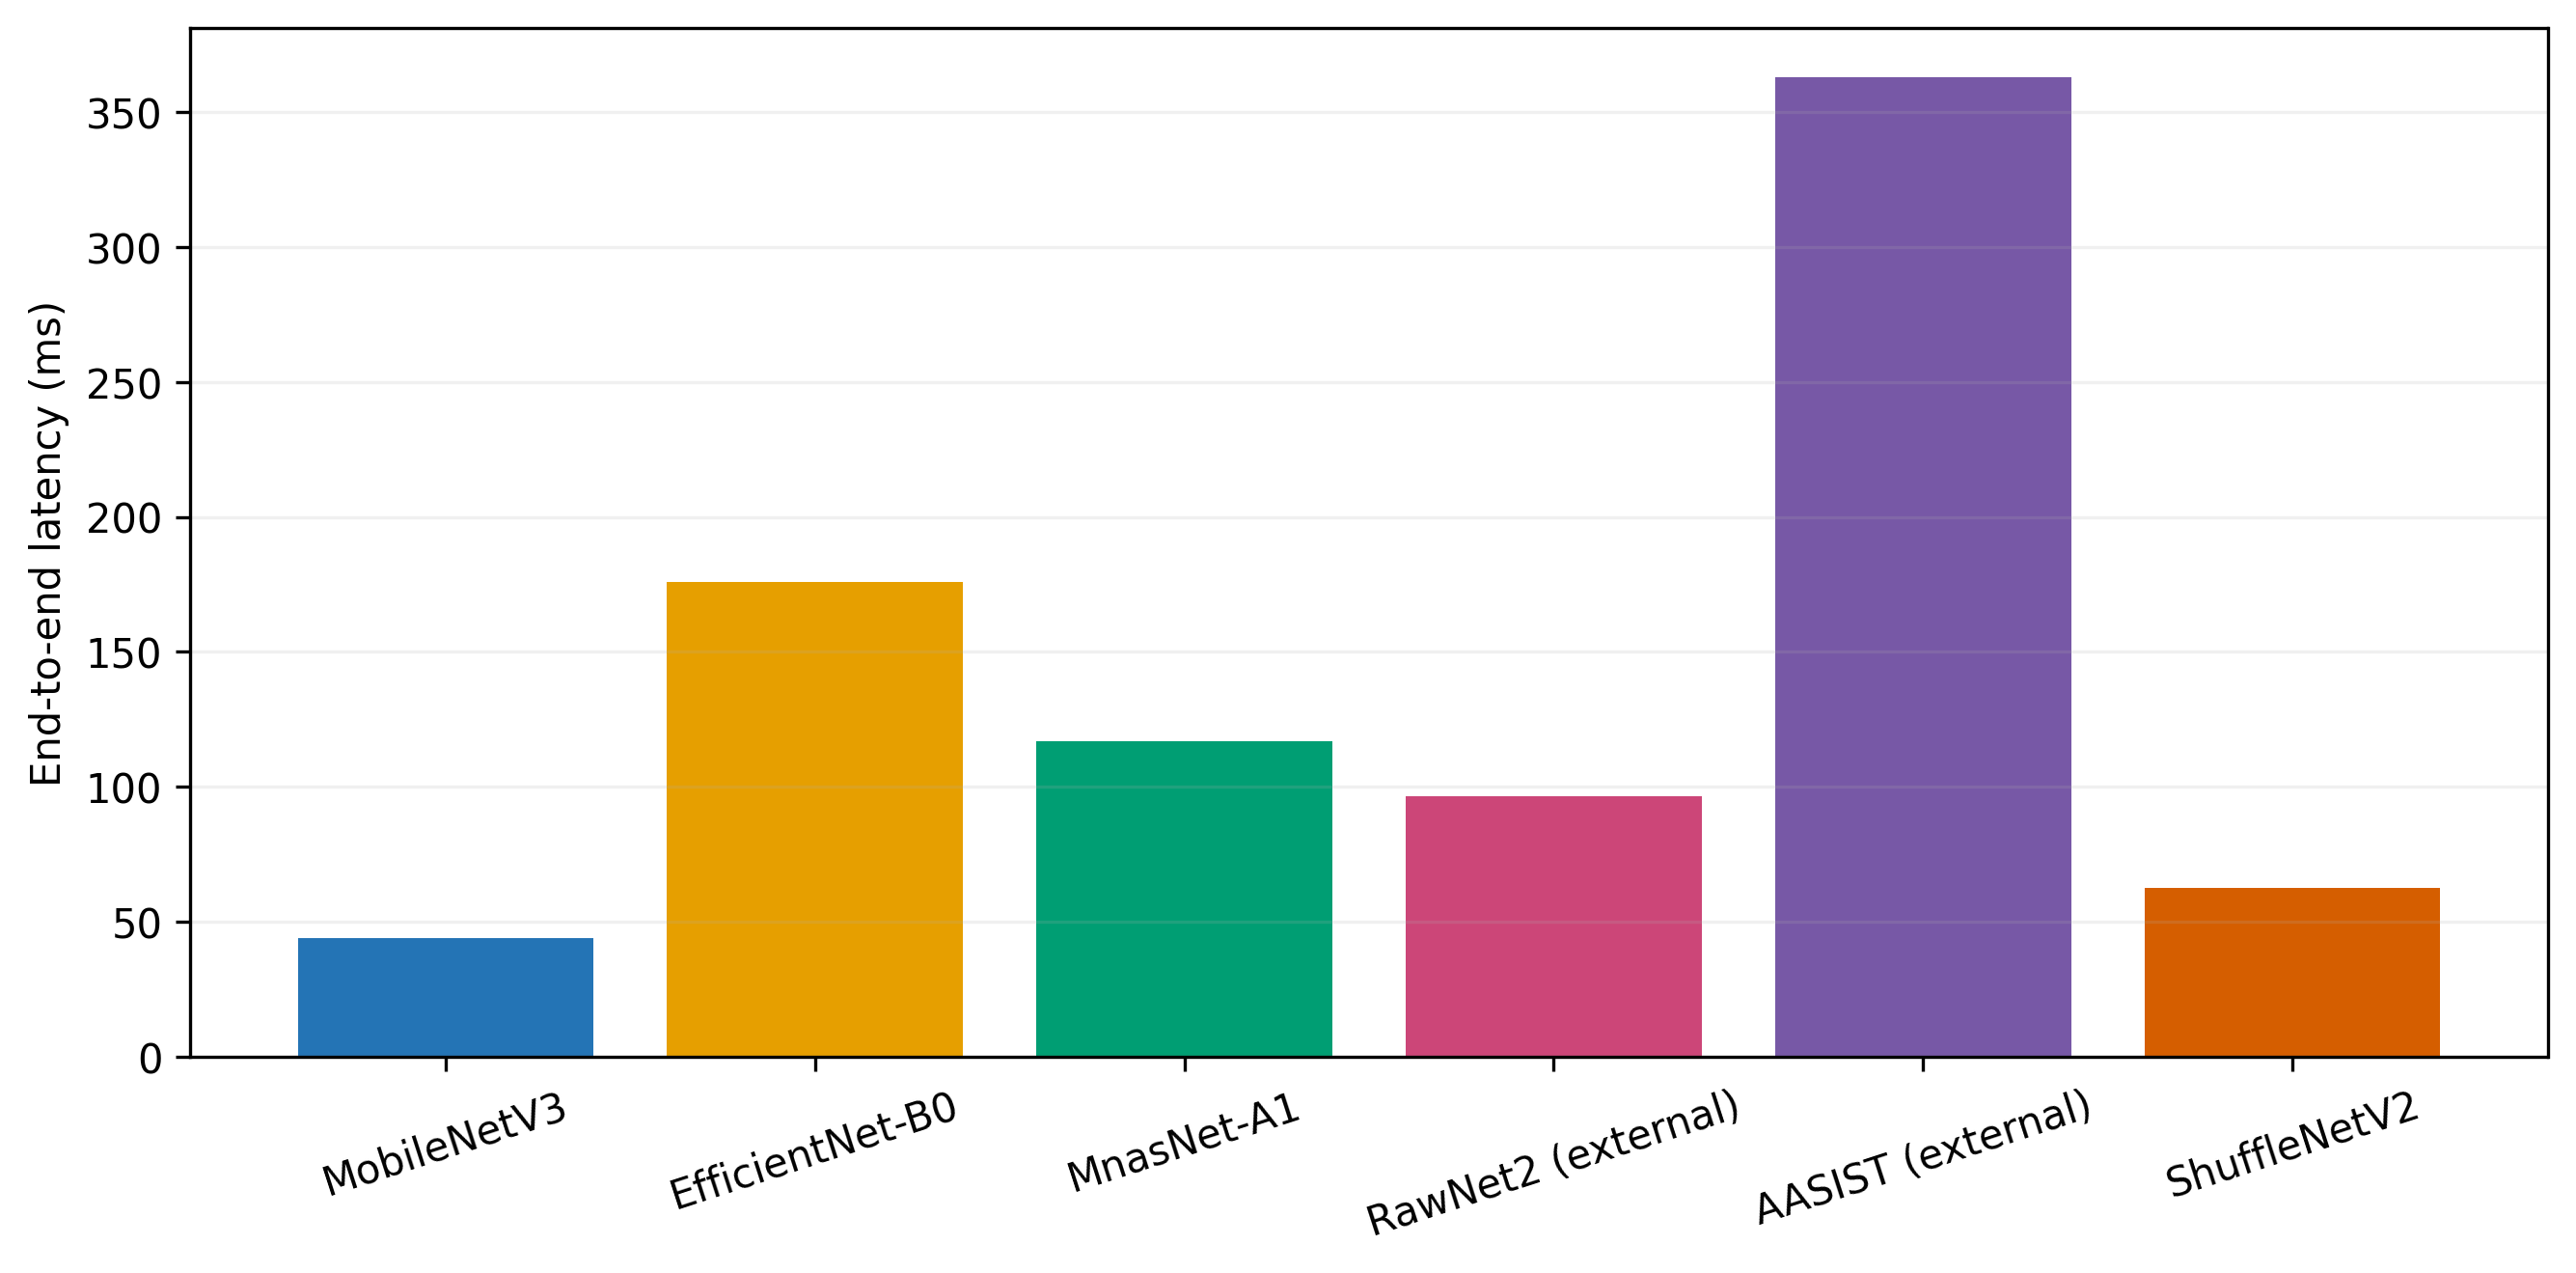
\includegraphics[width=\linewidth]{end_to_end_latency_bar_6_models.png}\\[-1mm]\small (a) Độ trễ đầu cuối
\end{minipage}\hfill
\begin{minipage}{.49\textwidth}\centering
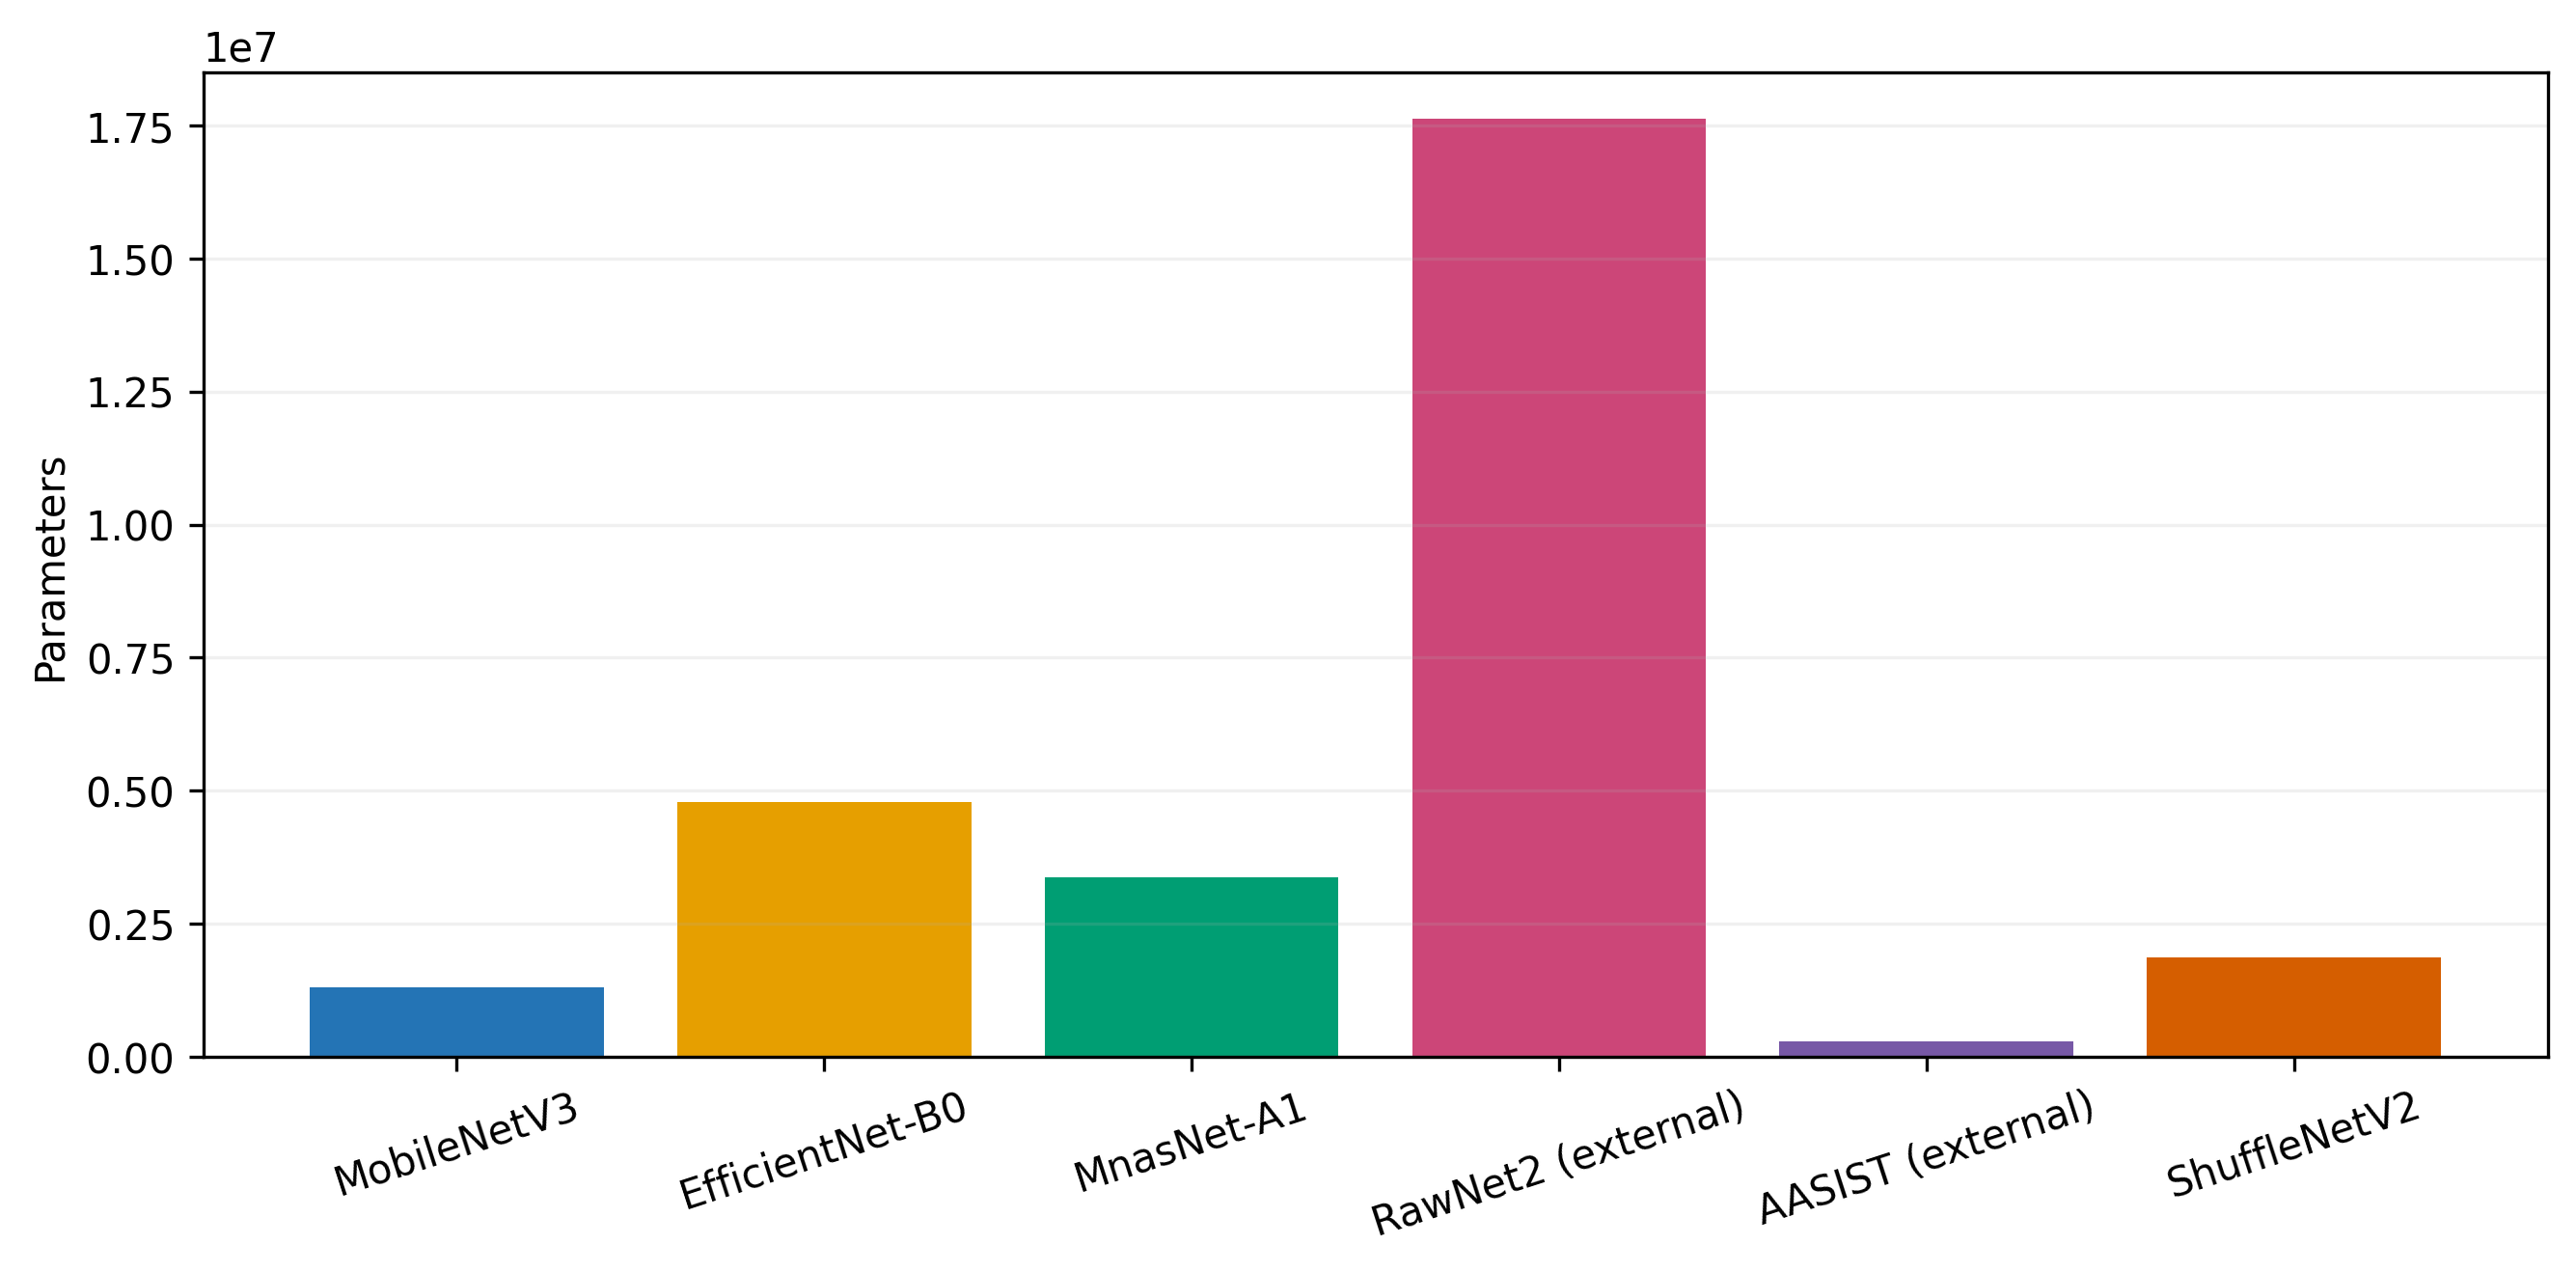
\includegraphics[width=\linewidth]{parameters_bar_6_models.png}\\[-1mm]\small (b) Số tham số
\end{minipage}
\caption{Thời gian chạy và độ phức tạp có liên quan nhưng không thể thay thế cho nhau.}
\label{fig:efficiency}
\end{figure}
Tất cả RTF đo được đều dưới 0,1, qua đó hỗ trợ suy luận ngoại tuyến nhanh hơn thời lượng âm thanh trên CPU này, chứ không xác nhận truyền luồng liên tục hay triển khai biên.

RSS của toàn tiến trình dao động từ 249,5 MiB đối với RawNet2 đến 651,2 MiB đối với EfficientNet. MobileNet và ShuffleNet lần lượt sử dụng 554,6 và 501,8 MiB, dù các artifact tuần tự hóa chỉ có kích thước 5,64 và 7,74 MiB; framework và trạng thái bộ cấp phát chi phối sự khác biệt này. Phần chênh P95 so với trung bình là 8,31 ms đối với MobileNet, 12,85 ms đối với ShuffleNet, 21,96 ms đối với MnasNet, 20,26 ms đối với EfficientNet, 6,08 ms đối với RawNet2 và 35,54 ms đối với AASIST. Các phân phối này củng cố sự cần thiết phải báo cáo cả độ trễ đuôi lẫn độ trễ trung bình.

\subsection{Các đánh đổi Pareto (RQ3)}
Tập chẩn đoán không bị trội gồm MobileNet, ShuffleNet và AASIST (Bảng~\ref{tab:pareto}, Hình~\ref{fig:pareto}). MobileNet cung cấp RTF thấp nhất; ShuffleNet kết hợp cùng EER trên tập con với mức suy giảm thấp hơn, đổi lại độ trễ tăng vừa phải. AASIST chỉ còn không bị trội vì mức suy giảm âm từ một đường cơ sở sạch yếu nằm tại một tọa độ cực trị. Việc thuộc biên không phải là một thứ hạng vô hướng. Theo các mục tiêu này, ShuffleNet trội hơn MnasNet và RawNet2; MobileNet trội hơn EfficientNet.

Bốn mô hình nhẹ đầu tiên có cùng EER chẩn đoán trên tập con là 0,0476, vì vậy quan hệ biên của chúng được quyết định bởi suy giảm độ bền vững và RTF. ShuffleNet cải thiện mức suy giảm trung bình 0,1476 so với MobileNet nhưng làm RTF tăng 0,0062; không mô hình nào trội hơn mô hình còn lại. MnasNet có mức suy giảm thấp hơn MobileNet một chút nhưng kém hơn về RTF và không cải thiện EER so với ShuffleNet, trong khi EfficientNet kém hơn MobileNet ở cả suy giảm lẫn RTF. Các phát biểu này áp dụng cho vector mục tiêu cố định và không ngụ ý một phương án triển khai ưu tiên khi chưa có các ràng buộc ứng dụng.

\begin{table}[!t]
\centering
\footnotesize
\caption{Kết quả Pareto thăm dò với ba mục tiêu trong phạm vi chẩn đoán.}
\label{tab:pareto}

\begin{tabular*}{\textwidth}{
@{\extracolsep{\fill}}
l
r
r
r
c
}
\toprule
Mô hình & EER tập con & $\Delta$F1 TB & RTF & Thuộc biên \\
\midrule
MobileNetV3     & .0476 & .3099 & .0146 & Có \\
ShuffleNetV2    & .0476 & .1623 & .0208 & Có \\
MnasNet-A1      & .0476 & .2989 & .0390 & Không \\
EfficientNet-B0 & .0476 & .3650 & .0586 & Không \\
RawNet2 ext.    & .4138 & .2241 & .0239 & Không \\
AASIST ext.     & .3810 & $-.0402$ & .0899 & Có \\
\bottomrule
\end{tabular*}

\end{table}

\begin{figure}[!t]
\centering
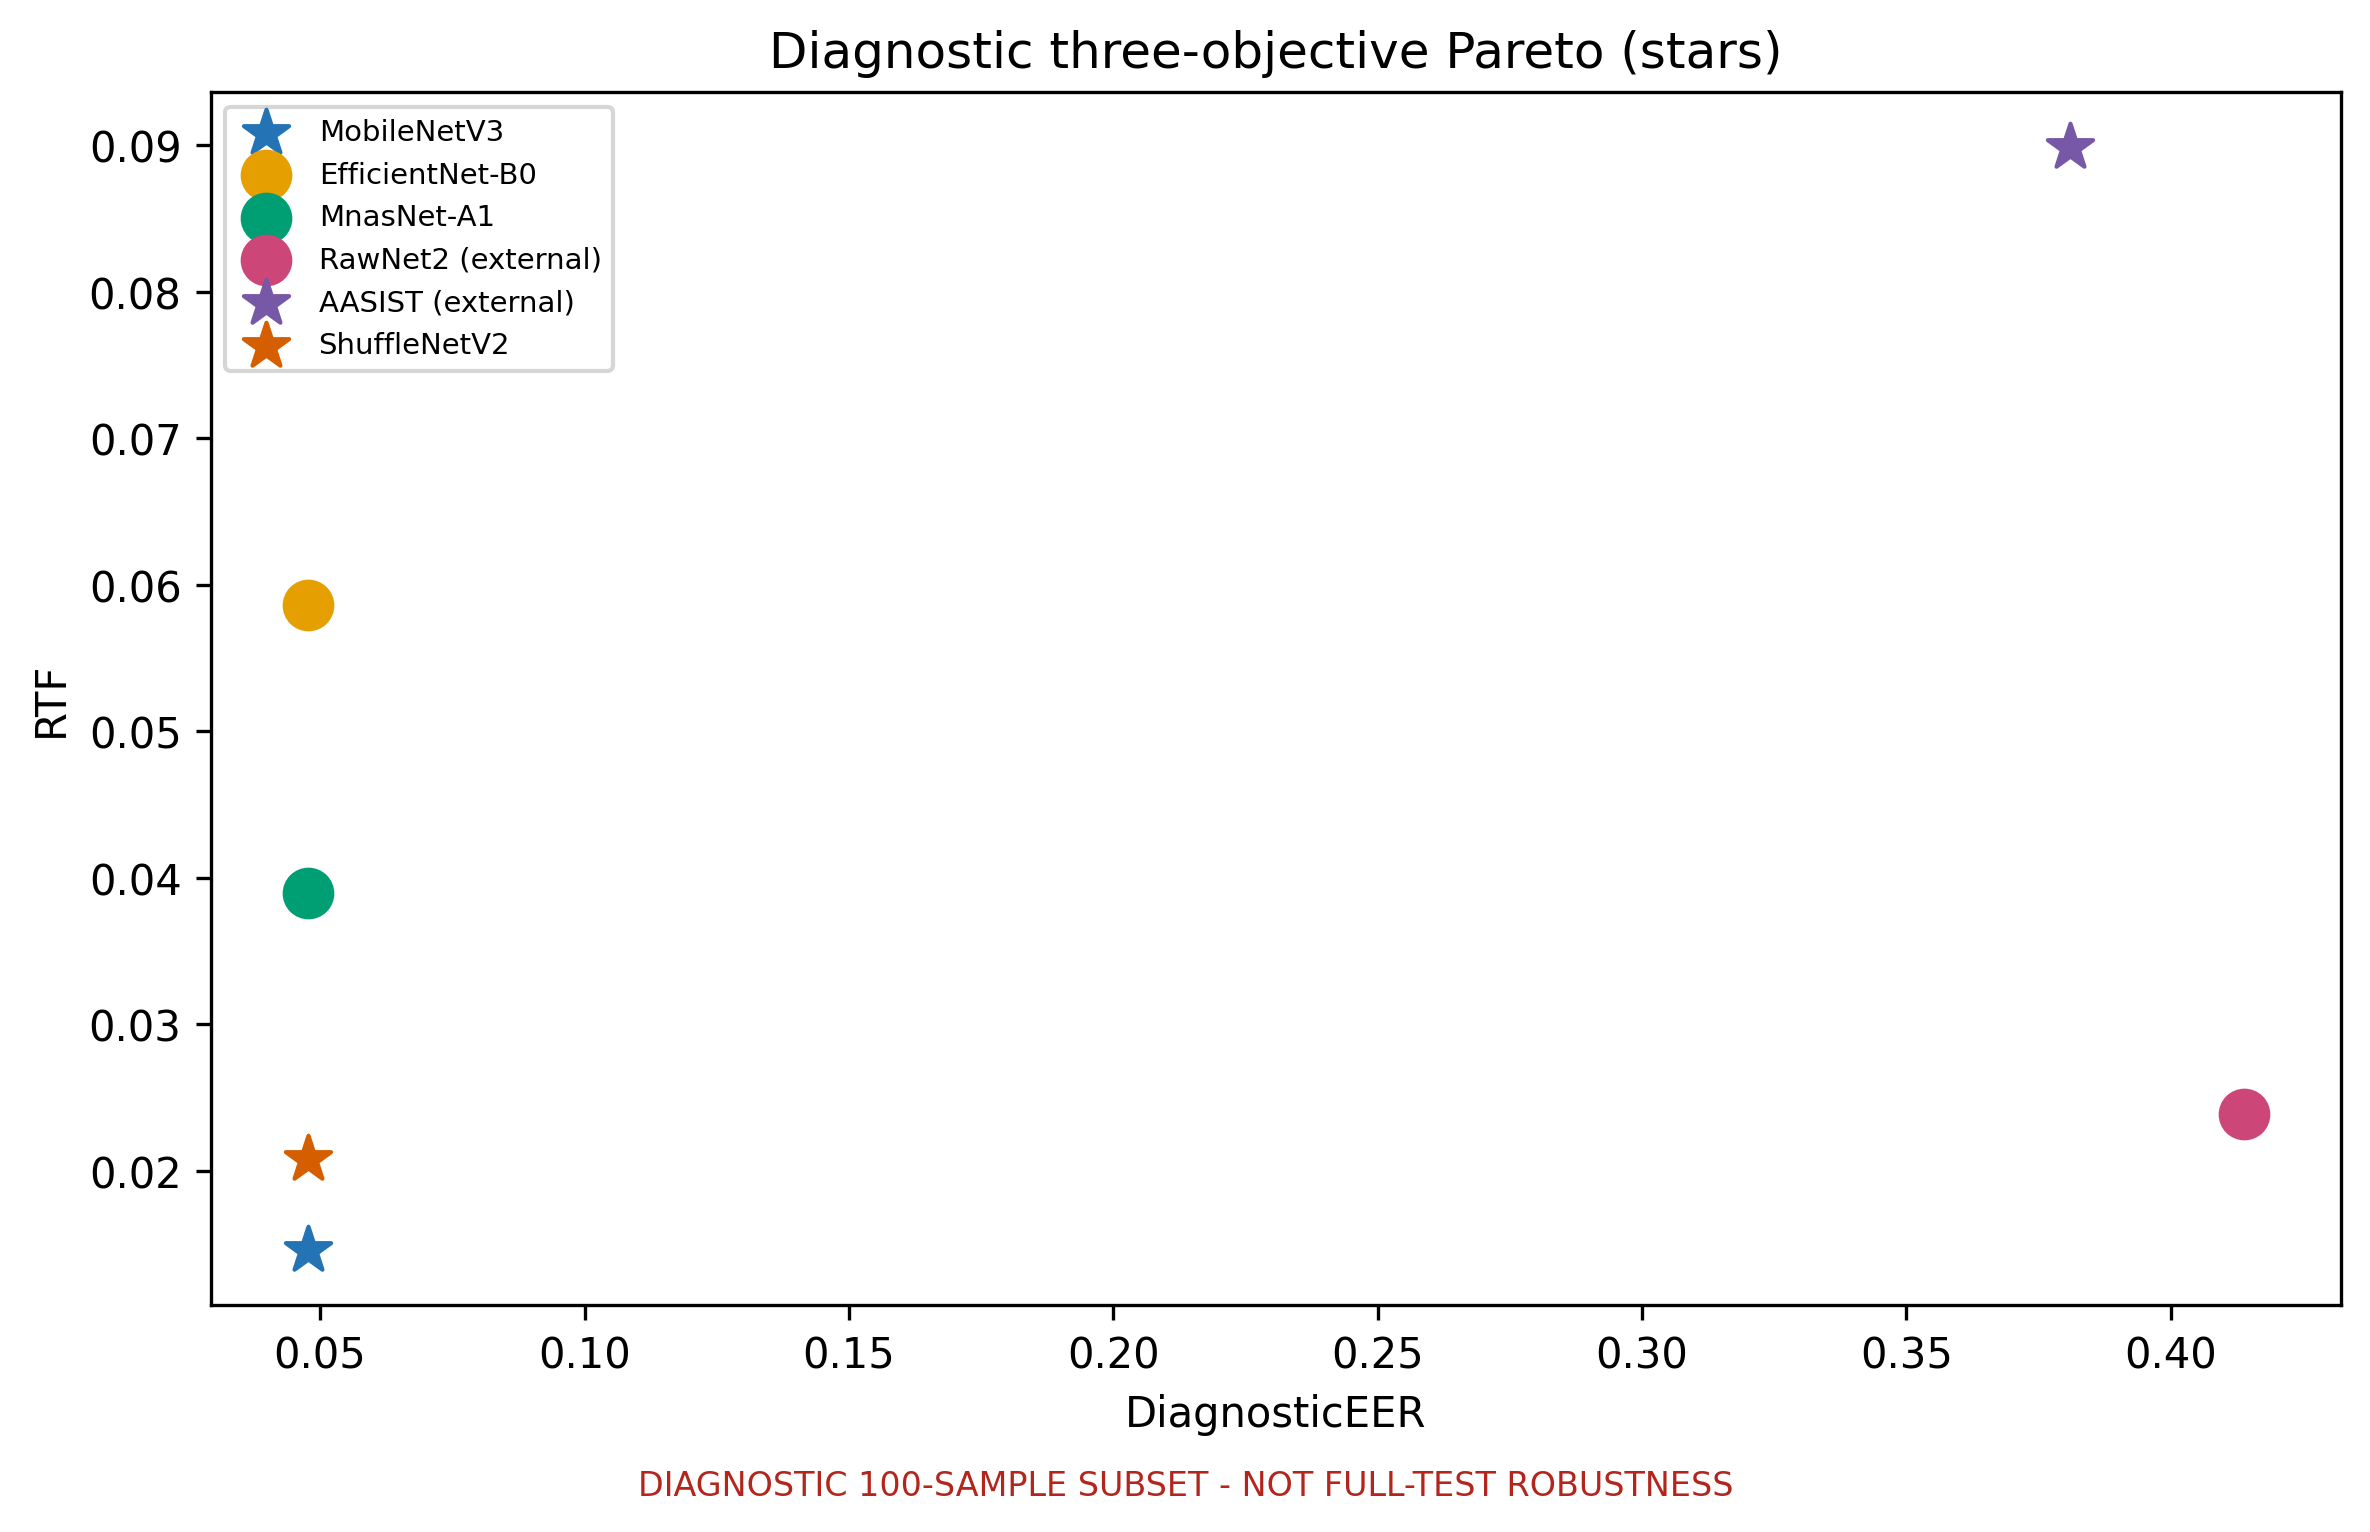
\includegraphics[width=.72\textwidth]{pareto_eer_rtf_6_models.png}
\caption{Phép chiếu EER--RTF; các dấu sao biểu thị biên chẩn đoán ba mục tiêu.}
\label{fig:pareto}
\end{figure}
Do độ bền vững chỉ mang tính chẩn đoán, RQ3 có tính thăm dò. Một lượt kiểm thử áp lực trên toàn bộ tập kiểm thử, phần cứng mới hoặc một chính sách ngưỡng khác đều có thể làm thay đổi biên.

\subsection{Phân tích lỗi, mức đồng thuận và bằng chứng thống kê}
Cả sáu bộ phát hiện đều dự đoán đúng trên 911 mẫu sạch và sai trên 10 mẫu. Bốn mô hình nhẹ đồng loạt dự đoán đúng trong khi cả hai mô hình tham chiếu dự đoán sai trên 785 mẫu; tình huống ngược lại xảy ra trên ba mẫu. ShuffleNet đồng thuận với MobileNet/EfficientNet/MnasNet ở 0,979/0,970/0,977 số quyết định, nhưng chỉ đồng thuận với RawNet2/AASIST ở 0,494/0,559; đồng thuận không đồng nghĩa với chính xác.

Các khoảng bootstrap 95\% trên toàn bộ tập kiểm thử của ShuffleNet là [0,9768, 0,9875] đối với F1, [0,9894, 0,9960] đối với AUC và [0,0103, 0,0207] đối với EER. Trong họ 15 cặp McNemar, ShuffleNet khác MobileNet sau hiệu chỉnh Holm ($p_{adj}=0.0096$), và khác mạnh hơn so với EfficientNet và MnasNet. MobileNet--MnasNet ($p_{adj}=0.1060$) và EfficientNet--MnasNet ($p_{adj}=0.1180$) không có ý nghĩa thống kê ở mức 0,05; mọi so sánh giữa mô hình nhẹ và mô hình tham chiếu đều có ý nghĩa thống kê. Các khoảng đầy đủ của sáu mô hình, chênh lệch F1 theo cặp, giá trị $p$ đã hiệu chỉnh, ma trận đồng thuận và ma trận lỗi được lưu trong các artifact bổ sung.

Để đầy đủ, các khoảng F1 tương ứng là [0,9654,0,9788] đối với MobileNet, [0,9573,0,9717] đối với MnasNet, [0,9477,0,9651] đối với EfficientNet, [0,5150,0,5489] đối với RawNet2 và [0,4928,0,5349] đối với AASIST. Các khoảng AUC lần lượt là [0,9871,0,9947], [0,9842,0,9923], [0,9833,0,9917], [0,4944,0,5395] và [0,5377,0,5815]. Những khoảng này định lượng biến thiên lấy mẫu của tập kiểm thử hữu hạn, với điều kiện là các checkpoint hiện có; chúng không thể đo biến thiên do seed huấn luyện.

Các khoảng EER là [0,0178,0,0311] đối với MobileNet, [0,0250,0,0379] đối với MnasNet, [0,0311,0,0482] đối với EfficientNet, [0,4616,0,5016] đối với RawNet2 và [0,4279,0,4660] đối với AASIST. Các khoảng chênh lệch F1 theo cặp của ShuffleNet trừ MobileNet/EfficientNet/MnasNet lần lượt là [0,0036,0,0166], [0,0182,0,0339] và [0,0116,0,0247]. Số lượng quyết định đúng bất đồng tương ứng (ShuffleNet sai/đúng) là 17/40, 12/71 và 10/52. Chiều chênh lệch và bằng chứng theo cặp phù hợp với bảng kết quả sạch, trong khi các so sánh MobileNet--MnasNet và EfficientNet--MnasNet không có ý nghĩa thống kê cho thấy không nên xếp hạng quá mức các hệ thống nhẹ ở nhóm giữa.

Phân tích phần giao bổ sung một góc nhìn hệ thống. Việc đồng loạt dự đoán đúng trên 911 bản ghi cho thấy một miền cốt lõi mà mọi artifact đều xử lý được bất chấp khác biệt về nguồn gốc, trong khi 10 lỗi đồng loạt xác định các ứng viên cần kiểm tra ở cấp dạng sóng, siêu dữ liệu và bộ sinh. Có 785 trường hợp mọi bộ phát hiện nhẹ đều đúng còn cả hai mô hình tham chiếu đều sai, chi phối bất đồng giữa hai nhóm; chỉ ba mẫu thể hiện mô thức ngược lại. Sự bất đối xứng này phù hợp với khả năng thích nghi theo tập dữ liệu, nhưng do thiếu chú thích nguồn/bộ sinh nên không thể xác lập các yếu tố âm học nào gây ra lỗi. Vì vậy, các nghiên cứu lỗi trong tương lai nên làm giàu manifest thay vì xem riêng sự bất đồng là một giải thích nhân quả.

Từ góc độ triển khai, MobileNet và ShuffleNet xác định miền đo được hấp dẫn nhất trong thực tiễn: cả hai kết hợp khả năng phân biệt cao trên dữ liệu sạch với RTF dưới 0,021, trong khi ShuffleNet cho kết quả độ bền vững sạch và chẩn đoán tốt hơn với chi phí độ trễ tăng vừa phải. Artifact lớn hơn và độ trễ cao hơn của EfficientNet không cải thiện chất lượng sạch trong trạng thái khởi động hiện có. MnasNet vẫn cạnh tranh về khả năng phát hiện nhưng bị trội theo các mục tiêu chẩn đoán hiện tại. Các hệ thống tham chiếu vẫn hữu ích về mặt khoa học như các phép thử áp lực không đồng nhất cho adapter và hợp đồng điểm số, dù kết quả sạch tuyệt đối của chúng còn yếu. Các kết luận này cần được xem xét lại sau khi hiệu chỉnh mô hình tham chiếu trên tập xác thực, huấn luyện mô hình nhẹ với nhiều seed và đo trên phần cứng đích.

\begin{figure}[!t]
\centering
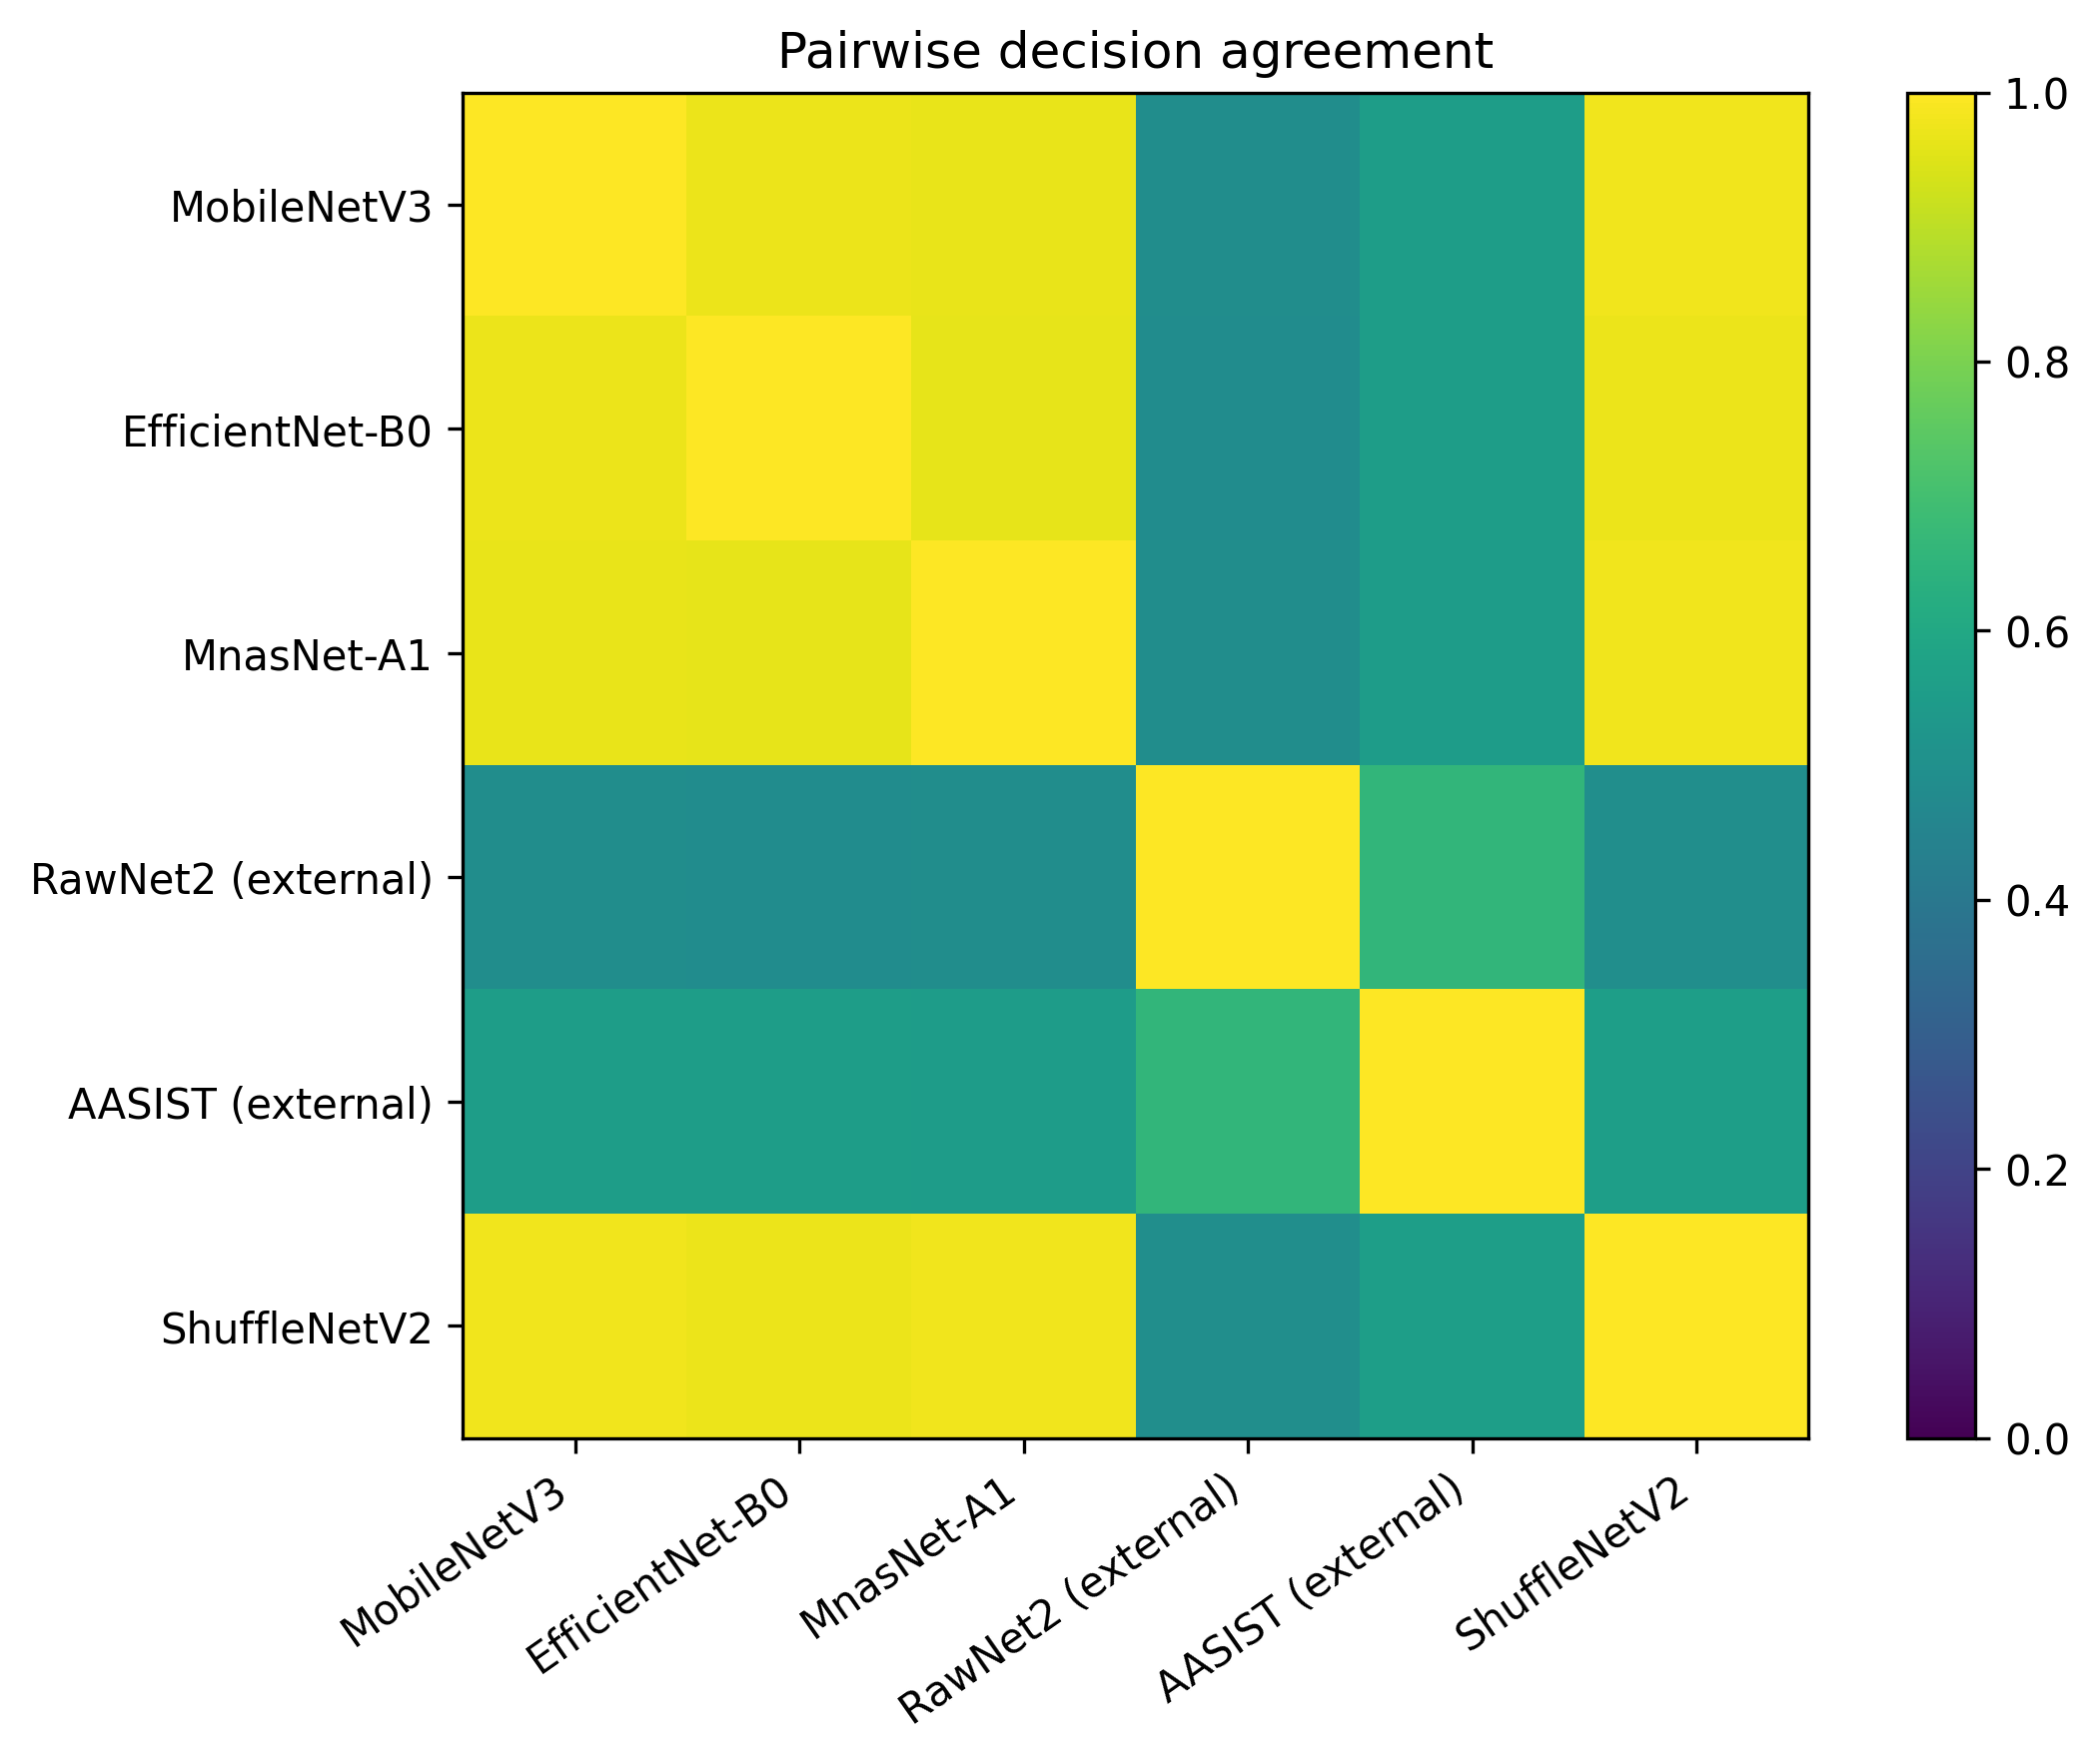
\includegraphics[width=.68\textwidth]{agreement_heatmap_6_models.png}
\caption{Mức đồng thuận theo cặp trên các ID mẫu giống nhau của toàn bộ tập kiểm thử; đồng thuận không phải là độ chính xác.}
\label{fig:agreement}
\end{figure}

\subsection{Trả lời trực tiếp các câu hỏi nghiên cứu}
\textbf{RQ1:} theo hợp đồng dữ liệu sạch này, bốn artifact nhẹ được huấn luyện cục bộ vượt trội hơn hai mô hình tham chiếu bên ngoài; ShuffleNet mạnh nhất về phát hiện còn MobileNet nhanh nhất. \textbf{RQ2:} những thay đổi do codec và phát lại mô phỏng nhỏ hơn so với nhiễu trắng SNR thấp, nhưng bằng chứng chỉ giới hạn ở 100 mẫu ghép cặp. \textbf{RQ3:} MobileNet, ShuffleNet và AASIST không bị trội trong không gian chẩn đoán; việc AASIST thuộc tập này phản ánh một tọa độ suy giảm âm chứ không phải khả năng phát hiện tuyệt đối mạnh. Các phát hiện này mô tả các artifact dưới LAVA, không khẳng định kiến trúc nào vượt trội một cách phổ quát.

\section{Hạn chế}
Nghiên cứu kết hợp học chuyển giao ImageNet (MobileNet/EfficientNet), tối ưu từ đầu (ShuffleNet/MnasNet) và các checkpoint RawNet2/AASIST bên ngoài, nên tính nhất quán trong đánh giá không đồng nghĩa với huấn luyện giống hệt nhau. Việc thiếu định danh người nói/nguồn/bộ sinh chỉ cho phép khẳng định các tập không giao nhau theo nhóm checksum. Đánh giá độ bền vững sử dụng 100 mẫu; phát lại là mô phỏng; không có corpus chưa thấy, phát lại vật lý, niêm phong phiên bản codec hay hiệu chỉnh xác suất. Thời gian chạy được đo trên một CPU máy tính để bàn thay vì thiết bị biên, và các checkpoint đơn lẻ cùng bootstrap trên tập kiểm thử không thay thế được huấn luyện nhiều seed. Công việc tương lai trước hết nên thực thi phép thử áp lực trên toàn bộ tập kiểm thử và một corpus bên ngoài giàu siêu dữ liệu, sau đó đo phát lại vật lý và phần cứng đích trước khi nghiên cứu lượng tử hóa hoặc truyền luồng.

\section{Kết luận}
LAVA cung cấp một giao diện có thể truy vết bằng chứng cho sáu artifact chống giả mạo giọng nói có kiến trúc không đồng nhất. Trên 2.737 bản ghi kiểm thử sạch, ShuffleNetV2-LSTM đạt F1/AUC/EER tốt nhất, trong khi MobileNetV3Small-LSTM giảm thiểu độ trễ và RTF. Các phép thử áp lực chẩn đoán xác định nhiễu SNR thấp là điểm yếu chính, còn phân tích đa mục tiêu giữ lại MobileNet, ShuffleNet và AASIST cho các đánh đổi khác nhau. Những kết quả này hỗ trợ so sánh hướng triển khai có khả năng tái lập và suy luận ngoại tuyến nhanh hơn thời lượng âm thanh, chứ không xác nhận miền chưa thấy, phát lại vật lý, truyền luồng hay thiết bị biên.

\section{Lời cảm ơn}
Nghiên cứu này nhận được sự hỗ trợ từ Đại học Kinh tế Thành phố Hồ Chí Minh, Việt Nam (UEH).

\bibliographystyle{IEEEtran}
\bibliography{references}
\end{document}
